\documentclass[12pt, oneside, a4paper]{book}

\usepackage{graphicx}
\usepackage{tikz-cd}
\usepackage{bm}
\usepackage{amsmath}
\usepackage{amssymb}
\usepackage{amsthm}
\usepackage{pgfplots}
\usepackage{xcolor}
\usepackage[shortlabels]{enumitem}
\usepackage[mathscr]{euscript}
\pgfplotsset{compat = newest}
\usepackage{float}
\usepackage{microtype}
\usepackage[mode=text]{siunitx}
\usepackage{longtable}
\usepackage{mathrsfs}
\graphicspath{
	{Figures/}
	{Figures/Chapter1/}
	{Figures/Chapter2/}
	{Figures/Chapter3/}
	{Figures/Chapter4/}
	{Figures/Chapter5/}
	{Figures/Appendix/}
}

\usepackage{vuwproposal} % sets up some local things, mostly the front page

\usepackage{palatino} % sets palatino as the default font

\usepackage{url} % for typesetting urls

\usepackage{booktabs} % for table creation

%\renewcommand{\baselinestretch}{1.00}


\begin{document} 
	
	
	\frontmatter
	% Book style knows about front matter
	% Report style doesn't so you need to set roman numbering etc yourself :-(
	
	%%%%%%%%%%%%%%%%%%%%%%%%%%%%%%%%%%%%%%%%%%%%%%%%%%%%%%%
	
	\title{Ordinal Pattern Features: Statistical Properties and Their Applications to Time Series Clustering}
	
	\author{Rasika Dilhani}
	\supervisors{Alejandro C.\ Frery, Andrea A.\ Rey and Nokuthaba Sibanda}
	
\subject{Data Science}
\abstract{%
	Time series analysis is central to understanding the dynamics of complex systems, yet classical time- and frequency-domain methods often rely on assumptions such as linearity, stationarity or Gaussianity that real-world data frequently violate. The ordinal-pattern approach introduced by Bandt and Pompe offers a non-parametric alternative: it maps local segments of a series to rank-based symbols and summarises their distribution with information-theoretic descriptors. The method is invariant to monotonic transformations, computationally inexpensive, and robust to outliers. Although these descriptors are widely used to characterise individual series, the joint use of a rich set of ordinal-pattern features as a basis for time series clustering and classification has received limited systematic attention.
	
	This thesis develops and evaluates a feature space of thirteen ordinal-pattern descriptors: the Shannon, R\'enyi and Tsallis entropies and the Fisher information measure; their associated statistical complexities; the disequilibrium; and variance-based measures of feature stability derived from the asymptotic distribution of the entropies. The descriptors are first studied through a simulation design based on convex combinations $X_t(w) = wX_t^{(S)} + (1-w)X_t^{(D)}$ of stochastic (AR(2), MA(2), ARMA(2,2)) and deterministic (logistic map, sine) processes. Varying the weight $w$ traces paths across the entropy--complexity plane and fills regions that pure models leave empty. Applying $k$-means to fifteen resulting model classes with series of length $n = 10\,000$ (embedding dimension $D = 4$) yields eleven clusters, selected by silhouette analysis, that largely correspond to the generating mechanisms; only borderline mixtures fall between neighbouring regimes. Clustering is poor for $n = 1000$. The three entropies prove almost perfectly correlated ($r \approx 0.99$), whereas the Fisher-based and variance-based features carry largely independent information.
	
	The features are then applied to two real-world problems. For Sentinel-1 SAR time series covering five land-cover classes, entropy, complexity and Fisher-based descriptors classified with a support vector machine reach sensitivities of 91.7\% (Forest) and 83.3\% (Agriculture), while Urban and Water remain difficult to separate. For RSAM seismic amplitude records at Whakaari, New Zealand (stations WIZ and WSRZ, 2014--2019), $k$-means and DBSCAN on weekly feature windows do not recover the Volcanic Alert Level classes (adjusted Rand index $< 0.06$). A class-weighted SVM recovers up to two of four eruption windows at WSRZ, which shows both the potential and the current limits of these features for detecting volcanic unrest.
	% [once completed I have to add: An event coincidence analysis further shows that ...]
	
	Overall, the thesis shows that ordinal-pattern features provide an interpretable, model-free representation that separates distinct dynamical regimes when series are sufficiently long. It also identifies the sample sizes, feature redundancies and application settings in which their discriminative power is limited.
}
	
	
	% Books don't normally have abstracts, and this is a bit of a hack
	
	% Uncomment the appropriate degree
	\phd
	%\mscthesisonly
	%\mscwithhonours
	%\mscbothparts
	% \otherdegree{DEGREE OR DIPLOMA NAME}
	
	
	
	%%%%%%%%%%%%%%%%%%%%%%%%%%%%%%%%%%%%%%%%%%%%%%%%%%%%%%%
	%New commands:
	
	\newcommand{\Sha}{\rotatebox[origin=c]{180}{$\Pi\kern-0.361em\Pi$}}
	\newcommand{\ot}{\otimes}
	\newtheorem{definition}{Definition}
	\newtheorem{theo}{Theorem}
	\newtheorem{contoh}{Example}
	\newtheorem{cor}{Corollary}
	\newtheorem{prop}{Proposition}
	\newtheorem{lemma}{Lemma}
	\newtheorem{remark}{Remark}
	\newtheorem{conjecture}{Conjecture}
	%%%%%%%%%%%%%%%%%%%%%%%%%%%%%%%%%%%%%%%%%%%%%%%%%%%%%%%
	
	\maketitle
	
	%\chapter*{Acknowledgments}\label{C:ack} 

Any acknowledgments should go in here, between the title page and the
table of contents.  The acknowledgments do not form a proper chapter,
and so don't get a number or appear in the table of contents.
	
	\tableofcontents
	
	
	%%%%%%%%%%%%%%%%%%%%%%%%%%%%%%%%%%%%%%%%%%%%%%%%%%%%%%%
	
	% book style knows about mainmatter
	% if you are using report style you will have to rest page numbering etc.
	\mainmatter
	
	%%%%%%%%%%%%%%%%%%%%%%%%%%%%%%%%%%%%%%%%%%%%%%%%%%%%%%%
	
	% individual chapters included here
	
%	% !TeX root = thesis.tex
\chapter{Introduction}\label{C:intro}

% =====================================================================
\section{Motivation}\label{S:intro:motivation}
% =====================================================================

A time series is a collection of observations $\{x_t\}$, each regarded as a realised value of a random variable $X_t$, indexed by discrete or continuous time.
Time series carry information about the system that generates them, and their analysis is central to engineering, economics and the physical, biological and Earth sciences.
Typical applications include the analysis of exchange rates and commodity prices in finance, the growth and decline of bacterial populations in biology, the spread of diseases such as COVID-19 or influenza in medicine, and the prediction of wet and dry days in geoscience (Figure~\ref{fig:timeseries}).

\begin{figure}[hbt]
	\centering
	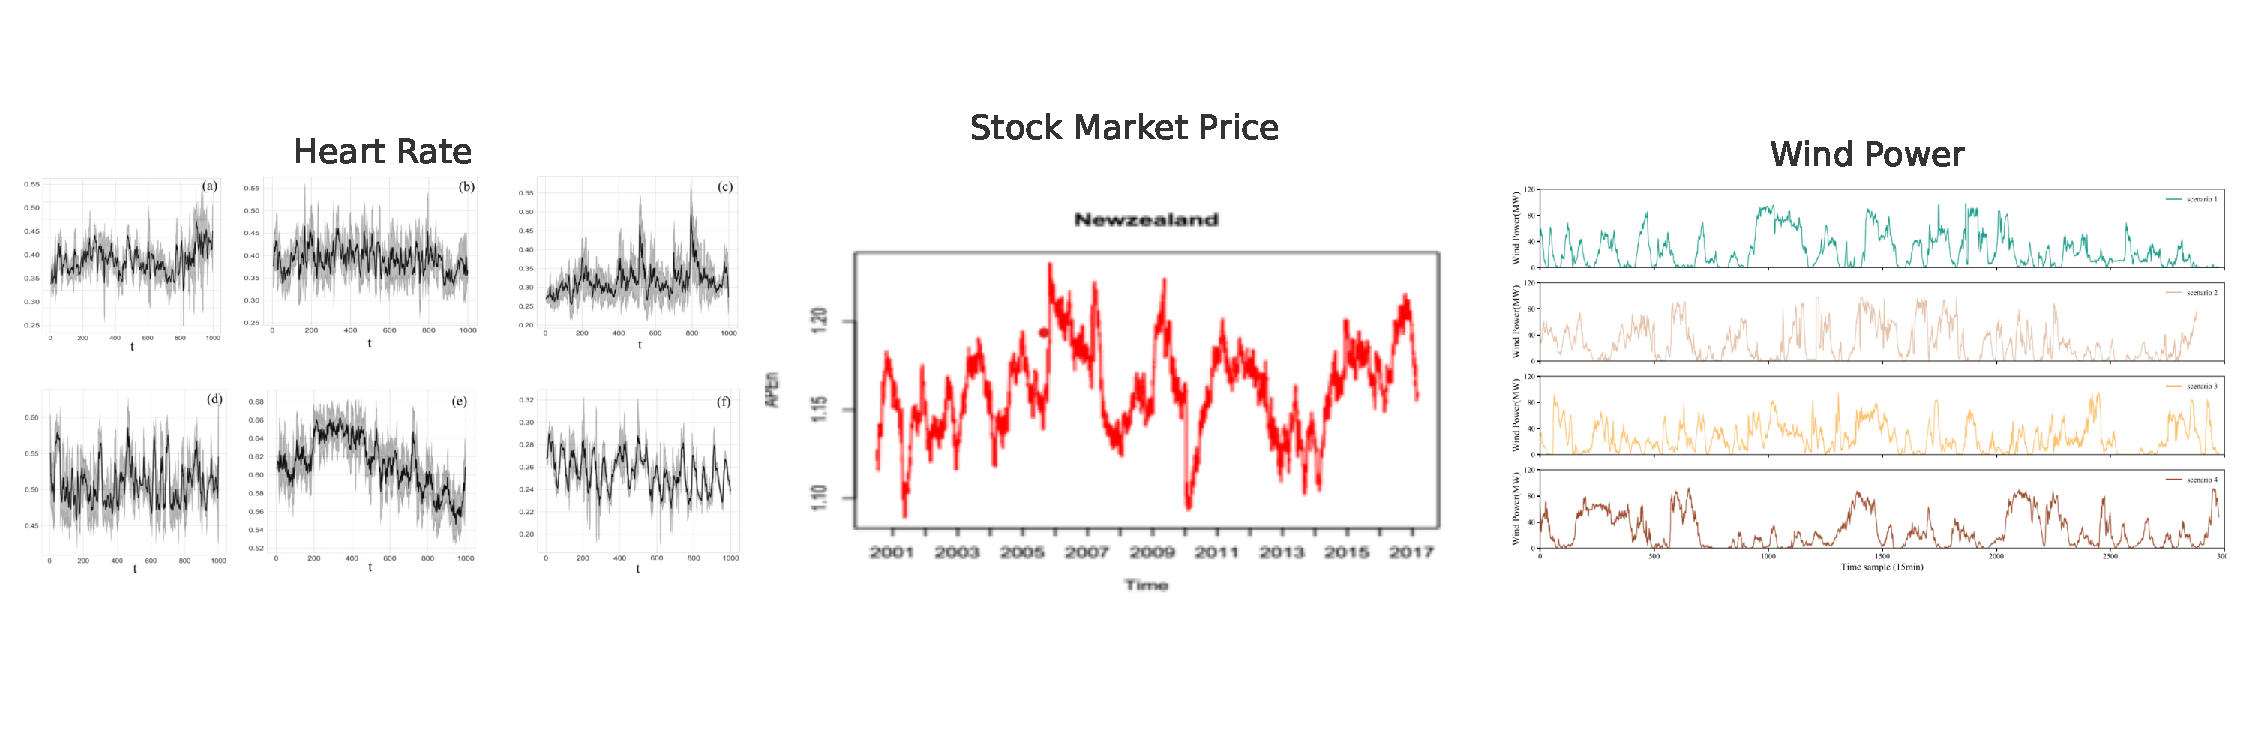
\includegraphics[width=0.99\textwidth]{Figures/Chapter1/time series plots}
	\caption{Examples of time series from biology, finance and geoscience. Sources: Silva et al., Patra et al.\ and Meng et al.~\cite{Silva2023,Patra2022,Meng2023}.}
	\label{fig:timeseries}
\end{figure}

The two classical families of methods are time-domain and frequency-domain analysis.
Time-domain methods, based on autocorrelation and regression, relate the present value of a series to its own past or to the past of other series.
Frequency-domain methods represent a series through spectral expansions such as Fourier modes or wavelets~\cite{treitel1995spectral}.
Both families typically rely on assumptions such as linearity, stationarity, Gaussianity or large sample sizes.
Real-world data frequently violate these assumptions: geophysical and remote-sensing records, for instance, are noisy, non-stationary, contain outliers and are often short relative to the phenomena of interest.
When the assumptions fail, the resulting inferences can be biased or misleading.

Classical non-parametric statistics address part of this problem by working with the ranks of the observations instead of their values, but most rank-based procedures ignore the temporal ordering that makes a time series informative.
Ordinal-pattern analysis, introduced by Bandt and Pompe~\cite{PhysRevLett.88.174102}, combines both ideas: it uses only the relative order of observations, and it does so locally, along the time axis.

% =====================================================================
\section{Ordinal patterns}\label{S:intro:op}
% =====================================================================

The Bandt and Pompe method transforms short, consecutive segments of a time series into symbols that encode the order relations among their values.
The empirical distribution of these symbols is then summarised by information-theoretic descriptors.
Because only order relations are used, the resulting distribution does not depend on any parametric model, is invariant to monotonic transformations of the data, and is robust to outliers and to observational noise.
The method is also computationally inexpensive.
Since 2002 it has been applied in biomedical signal processing, optical chaos, hydrology, geophysics, econophysics, engineering and biometrics, and to the assessment of pseudo-random number generators~\cite{Zanin2012}.

Formally, let $\bm{x}=(x_1,x_2,\dots,x_{n+D-1})$ be a real-valued time series of length $n+D-1$ without ties.
For an embedding dimension $D$ (usually $3\le D\le 6$) and unit time delay, each window $(x_j,\dots,x_{j+D-1})$, $1\le j\le n$, is mapped to one of the $D!$ possible permutations of $\{1,\dots,D\}$.
In this thesis each window is encoded by the vector of ranks of its values.
This yields the symbol sequence $\bm{\pi}=(\pi_1,\dots,\pi_n)$ with $\pi_j\in\{\pi^1,\dots,\pi^{D!}\}$, and the histogram of proportions $\bm{h}=(h_1,\dots,h_{k})$, $k=D!$, where $h_\ell$ is the proportion of symbols of type $\pi^\ell$.
For statistical purposes we model the symbol counts as a $k$-dimensional multinomial random vector.

% ---------------------------------------------------------------------
\subsection{An illustrative example}\label{S:intro:example}
% ---------------------------------------------------------------------

Consider the mean monthly relative humidity in Wellington (Table~\ref{tab:humidity} and Figure~\ref{fig:humidity}).

\begin{table}[hbt]
	\centering
	\begin{tabular}{lc}
		\toprule
		Month & Mean relative humidity (\%) \\
		\midrule
		January & 77.3 \\
		February & 81.0 \\
		March & 82.4 \\
		April & 81.7 \\
		May & 83.6 \\
		June & 85.6 \\
		July & 84.4 \\
		August & 83.1 \\
		September & 78.8 \\
		October & 79.6 \\
		November & 78.2 \\
		December & 78.8 \\
		\bottomrule
	\end{tabular}
	\caption{Mean monthly relative humidity in Wellington.}
	\label{tab:humidity}
\end{table}

\begin{figure}[hbt]
	\centering
	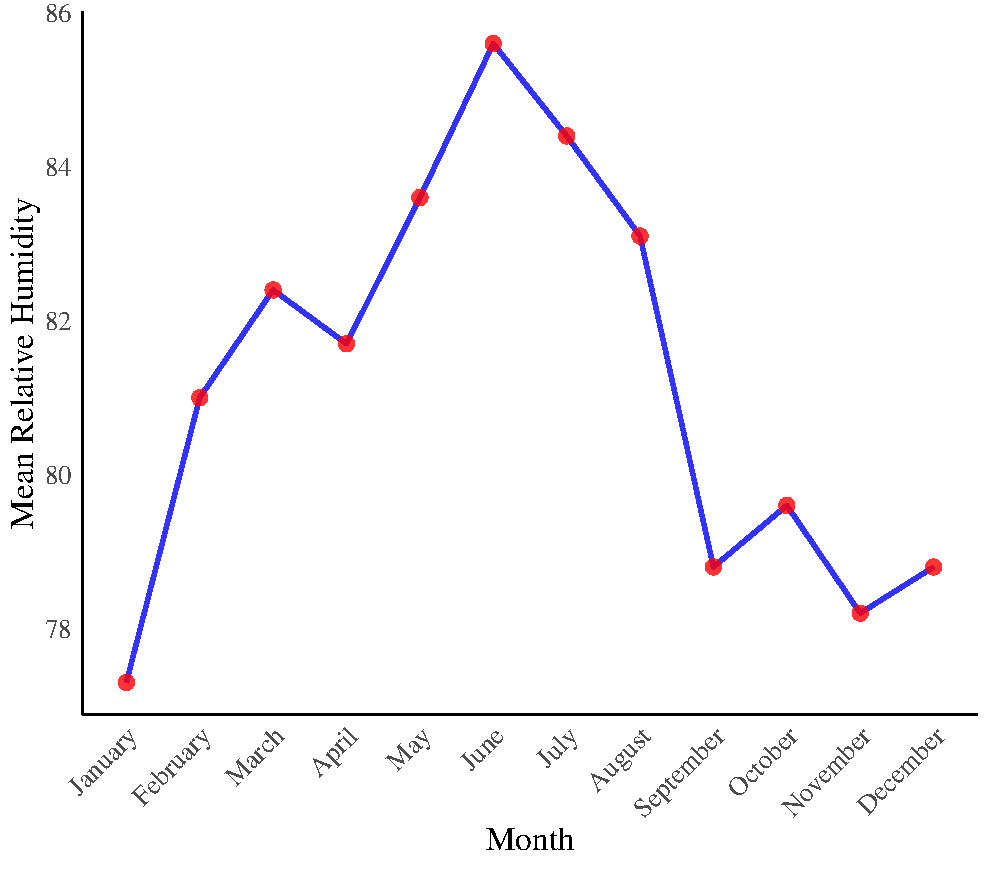
\includegraphics[width=0.6\textwidth]{Figures/Chapter1/humidity graph}
	\caption{Mean monthly relative humidity in Wellington.}
	\label{fig:humidity}
\end{figure}

With $D=3$, the first overlapping window $(77.3, 81.0, 82.4)$ is increasing: $77.3$ receives rank $1$, $81.0$ rank $2$ and $82.4$ rank $3$, giving the pattern $(123)$.
The window $(83.1, 78.8, 79.6)$ gives the pattern $(312)$, since $83.1$ is the largest value, $78.8$ the smallest and $79.6$ the intermediate one.
Proceeding in this way, the $12$ observations produce $n=10$ patterns (Table~\ref{tab:op}).

\begin{table}[hbt]
	\centering
	\begin{tabular}{lcr}
		\toprule
		$t$ & Window & Ordinal pattern \\
		\midrule
		1 & (77.3, 81.0, 82.4) & (123) $=\pi^1$\\
		2 & (81.0, 82.4, 81.7) & (132) $=\pi^2$\\
		3 & (82.4, 81.7, 83.6) & (213) $=\pi^3$\\
		4 & (81.7, 83.6, 85.6) & (123) $=\pi^1$\\
		5 & (83.6, 85.6, 84.4) & (132) $=\pi^2$\\
		6 & (85.6, 84.4, 83.1) & (321) $=\pi^6$\\
		7 & (84.4, 83.1, 78.8) & (321) $=\pi^6$\\
		8 & (83.1, 78.8, 79.6) & (312) $=\pi^5$\\
		9 & (78.8, 79.6, 78.2) & (231) $=\pi^4$\\
		10 & (79.6, 78.2, 78.8) & (312) $=\pi^5$\\
		\bottomrule
	\end{tabular}
	\caption{Ordinal patterns of dimension $D=3$ for the series in Table~\ref{tab:humidity}.}
	\label{tab:op}
\end{table}

The six possible patterns are $\{\pi^1,\dots,\pi^6\}=\{(123),(132),(213),(231),(312),(321)\}$, and their relative frequencies are
\begin{equation}
	\hat{p}_i=\frac{\#\{\pi_j\in\bm{\pi}:\pi_j=\pi^i\}}{n},\qquad 1\le i\le 6,
\end{equation}
giving $\hat{\bm{p}}=(2,2,1,1,2,2)/10$ (Table~\ref{tab:probability_function} and Figure~\ref{fig:histogram}).

\begin{table}[hbt]
	\centering
	\begin{tabular}{lc}
		\toprule
		Pattern & Relative frequency \\
		\midrule
		$\pi^1$ & $2/10$ \\
		$\pi^2$ & $2/10$ \\
		$\pi^3$ & $1/10$ \\
		$\pi^4$ & $1/10$ \\
		$\pi^5$ & $2/10$ \\
		$\pi^6$ & $2/10$ \\
		\bottomrule
	\end{tabular}
	\caption{Empirical distribution of ordinal patterns for the humidity series.}
	\label{tab:probability_function}
\end{table}

\begin{figure}[hbt]
	\centering
	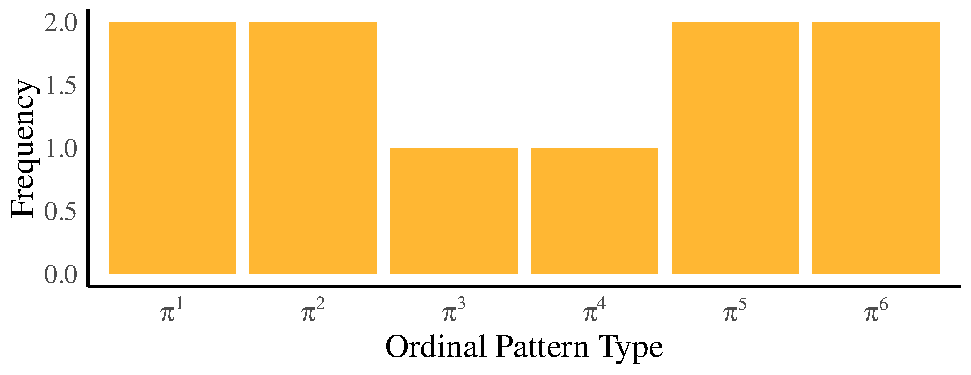
\includegraphics[width=0.6\textwidth]{Figures/Chapter1/frequency histogram}
	\caption{Histogram of the proportions of observed patterns (Table~\ref{tab:probability_function}).}
	\label{fig:histogram}
\end{figure}

All the features studied in this thesis are functions of distributions such as $\hat{\bm p}$.
In practice, much longer series are needed: with $D$ patterns there are $D!$ bins to estimate, and reliable estimation requires $n\gg D!$.

% =====================================================================
\section{From ordinal patterns to features}\label{S:intro:features}
% =====================================================================

Bandt and Pompe summarised $\hat{\bm p}$ by its normalised Shannon entropy, known as permutation entropy~\cite{PhysRevLett.88.174102}.
Entropy alone, however, does not distinguish all types of dynamics.
L\'opez-Ruiz et al.~\cite{lopez1995statistical} introduced statistical complexity as the product of entropy and a disequilibrium term measuring the distance to the uniform distribution.
Lamberti et al.~\cite{lamberti2004intensive} replaced the Euclidean distance with the Jensen--Shannon divergence, which gives an intensive measure.
Rosso et al.~\cite{Rosso2007} proposed representing each series as a point in the entropy--complexity ($H\times C$) plane, and Martin et al.~\cite{Martin2006} derived the curves that bound the attainable region of this plane.
Generalised entropies (R\'enyi and Tsallis) and the Fisher information measure, which is sensitive to local changes in the distribution, provide further descriptors.
Because all these features are estimated from finite samples, their sampling variability matters.
Rey et al.~\cite{Rey2024} derived the asymptotic distributions of the Shannon, R\'enyi and Tsallis entropies and of the Fisher information measure of ordinal patterns, which yield variances and confidence intervals for these quantities.

% =====================================================================
\section{Research gap and objectives}\label{S:intro:gap}
% =====================================================================

Ordinal-pattern descriptors are widely used to characterise individual time series, usually one or two at a time, and most often through permutation entropy alone.
Clustering based on ordinal-pattern distributions has been proposed~\cite{Brandmaier2015}.
However, the joint use of a rich set of ordinal-pattern features as a feature space for clustering and classification has received little systematic attention.
Such a feature space would combine several entropies, their complexities, the Fisher information and variance-based measures of stability.
In particular, it is not known:
\begin{itemize}
	\item how these features behave for processes that mix deterministic and stochastic dynamics, which occupy regions of the $H\times C$ plane that pure models do not reach;
	\item which features carry complementary information and which are redundant;
	\item how large a series must be for clustering in this feature space to recover the generating mechanisms;
	\item how well the features perform on real, noisy data from the Earth sciences.
\end{itemize}

The objectives of this thesis are therefore to:
\begin{enumerate}
	\item define a feature space of thirteen ordinal-pattern descriptors, comprising entropies, statistical complexities, the Fisher information measure, the disequilibrium and variance-based stability measures;
	\item study the behaviour of these features through a simulation design based on convex combinations of deterministic and stochastic processes, and assess their ability to support unsupervised clustering of time series;
	\item apply the features to land use/land cover classification of Synthetic Aperture Radar (SAR) time series;
	\item apply the features to the detection of unusual seismic-amplitude behaviour at Whakaari, New Zealand, and assess their relationship with Volcanic Alert Levels and eruptions.
	% \item [Optional, if completed] use event coincidence analysis to quantify the temporal association between feature anomalies and volcanic events.
\end{enumerate}

% =====================================================================
\section{Contributions}\label{S:intro:contrib}
% =====================================================================

The main contributions of this thesis are:
\begin{enumerate}
	\item \textbf{A simulation framework based on convex combinations.} Series of the form $X_t(w)=wX_t^{(S)}+(1-w)X_t^{(D)}$, $0\le w\le 1$, with stochastic components AR(2), MA(2) and ARMA(2,2) and deterministic components the logistic map and a sine function, trace continuous paths in the $H\times C$ plane. These paths populate regions that pure models leave empty.
	\item \textbf{Clustering in an ordinal-pattern feature space.} Fifteen model classes are clustered with $k$-means using the thirteen features. With $n=10\,000$ and $D=4$, the eleven clusters selected by silhouette analysis largely correspond to the generating mechanisms, while only borderline mixtures are split between neighbouring clusters. Clustering degrades markedly for $n=1000$.
	\item \textbf{An assessment of feature redundancy.} The Shannon, R\'enyi and Tsallis entropies are almost perfectly correlated, whereas the Fisher-based and variance-based features carry largely independent information.
	\item \textbf{An application to SAR land cover classification.} Ordinal-pattern features combined with a support vector machine separate Agriculture and Forest well, while Urban and Water remain difficult to distinguish.
	\item \textbf{An application to volcano monitoring.} At Whakaari, unsupervised clustering of weekly RSAM feature windows does not recover the Volcanic Alert Level classes, and supervised classification recovers only some eruption windows. The analysis quantifies both the potential and the current limits of ordinal-pattern features for detecting volcanic unrest.
\end{enumerate}

Parts of this work have been presented in the following publication:
\begin{itemize}
	\item R.~Dilhani, A.~Sabir, U.~Khati, A.~C.~Frery and A.~A.~Rey, ``Land cover classification in SAR time series using ordinal pattern features,'' [venue, year].
\end{itemize}

% =====================================================================
\section{Thesis outline}\label{S:intro:outline}
% =====================================================================

The remainder of this thesis is organised as follows.
Chapter~\ref{C:lit} reviews the literature on ordinal-pattern analysis, information-theoretic quantifiers and their applications to time series clustering and to geophysical and remote-sensing data.
Chapter~\ref{C:features} defines the thirteen ordinal-pattern features, including the Shannon, R\'enyi and Tsallis entropies, the Fisher information measure, the associated statistical complexities and the asymptotic variances used to quantify their stability.
Chapter~\ref{C:sim} presents the convex-combination simulation study and the clustering of simulated time series in the ordinal-pattern feature space.
Chapter~\ref{C:sar} applies the features to land use/land cover classification of SAR time series.
Chapter~\ref{C:seismic} analyses RSAM seismic-amplitude records from Whakaari.
% Chapter~\ref{C:eca} applies event coincidence analysis to ... [optional]
Chapter~\ref{C:concl} summarises the findings, discusses limitations and outlines directions for future research.
%	% !TeX root = thesis.tex
\chapter{Literature Review}\label{C:lit}

The analysis of complex time series has long relied on both time-domain and frequency-domain techniques. 
However, traditional methods often fall short in capturing nonlinear dynamics or are limited by strict assumptions such as stationarity and Gaussianity. 

The ordinal symbolic approach introduced by Bandt and Pompe in 2002 marked a significant theoretical advance by enabling robust, model-free characterization of time series. 
Their approach, rooted in information theory, involves converting segments of time series data into symbols based on the ordinal (rank) relationships among the data points.
These symbols are called "ordinal patterns." After computing all the symbols, their relative frequencies are used to estimate the probability distribution of ordinal patterns.

From this distribution estimate, two key descriptors entropy and complexity are calculated to characterize the time series: the scaled Shannon entropy, now widely known as permutation entropy, and the statistical complexity.

This chapter is divided into four main sections. Section~\ref{Sec:Onset} presents a brief overview of the area, focusing on what we consider the four seminal papers. Section~\ref{Sec:ResearchQuestion} discusses the research question and the motivation for conducting the bibliometric analysis. The final section, Section~\ref{Sec:BiblioIntro}, highlights the importance of bibliometric analysis and presents the results obtained from references that cite the Bandt and Pompe methodology and other related topics based on our research focus. 
Section~\ref{Sec:StatisitcalProperty} discusses the statistical properties of features from ordinal patterns based on the literature review.   

\section{The Onset of the Entropy-Complexity Plane}\label{Sec:Onset}

This section discusses the emergence of the entropy-complexity plane. This topic is presented as a central theme because it reflects the foundation of our main research focus and illustrates how it has evolved over time into the current approach to time series analysis based on the concept of ordinal patterns. 

López-Ruiz et al.~\cite{lopez1995statistical} to capture the structure of a system:
the product between the entropy and a distance between the estimated model and a non-informative model is an interesting way of measuring complexity.
Lamberti et al.~\cite{lamberti2004intensive}, using that idea, proposed using the Euclidean distance between the measured probability function and the uniform distribution.
Rosso et al.~\cite{EEGAnalysisUsingWaveletBasedInformationTools} discussed using other distances, proposed the Jensen-Shannon distance, and used it jointly with the scaled Shannon entropy to form a bivariate feature.
They mapped this feature into the so-called ``Entropy-Complexity Plane,'' devising  a powerful diagnostic tool to distinguish between different dynamical regimes, such as chaos, noise, and periodicity.
Further, Martin et.al.~\cite{Martin2006} discussed the boundaries of this generalized statistical complexity measure. 

In the following, we present the research question and the motivation for continuing this research. 

\section{Research Question and Motivation}\label{Sec:ResearchQuestion}

The primary research question guiding this study is:
\begin{quote}
	\textit{How can confidence intervals for generalized entropy measures (Shannon, Tsallis, Rényi, Fisher information measure) and their associated complexity metrics be used to improve the robustness and discriminative power of time series clustering techniques?}
\end{quote}

We are motivated to conduct a literature review to confirm the relevance of our research areas in relation to the research question. Our aim is to determine whether other researchers are engaging with similar types of questions. Additionally, we seek to verify whether there is a strong focus on practical applications within this topic. 


\section{The Bibliometric Analysis: data collection, tools and background}\label{Sec:BiblioIntro}

Bibliometric analyses provide a quantitative approach to reviewing and mapping the intellectual structure of a research field. By systematically analyzing citation patterns, author collaborations, and keyword co-occurrences, they help identify key themes, research trends, and emerging topics. This method ensures objectivity, reveals key contributions, and offers a structured overview of intellectual development, making it a valuable tool for systematic literature reviews.

In this study, we conducted a bibliometric analysis using the Bibliometrix package in R and its user-friendly web interface Biblioshiny~\cite{Aria2017} focusing on literature related to ordinal patterns, permutation entropy, and complexity measures in time series analysis. 

Section~\ref{Subsec:Dataextraction} discusses the data extraction process using the Bibliometrix package in R.

\subsection{Conceptual Structure: Data extraction and Summary Statistics}\label{Subsec:Dataextraction}

Scopus-indexed references that cited the seminal work by Bandt and Pompe, along with other references relevant to our research topic, were collected on June 9, 2025.
Based on these reference files, we analyzed a dataset consisting of 4125 reference files spanning the years 1993 to 2025. 
The descriptive analysis of the dataset revealed a total of 4063 usable documents (out of 4125; the others had missing data and were removed), sourced from 1317 publication sources. 
The dataset shows an annual growth rate of \SI{18.15}{\percent}, involving 7254 authors, 
123 single-authored documents, \SI{27.32}{\percent} international co-authorship, 
with an average of 4.28 co-authors per document. 
The author keywords totaled 7667, 
with an average document age of 5.7 years, and 22.6 citations per document. 

\subsection{Thematic Map Analysis}

Thematic map helps to understand the research direction and the relevant topics for the future studies. Therefore, we motivated to analyse it. The axes of the thematic map depicts the strength of their internal (density), which reflects inter-cluster growth, and external (connectivity) relevance or significance of the study in a particular area (centrality). 

Figure~\ref{fig:ThematicMap} illustrates the thematic map derived from author keywords.

\begin{figure}[H]
	\centering
	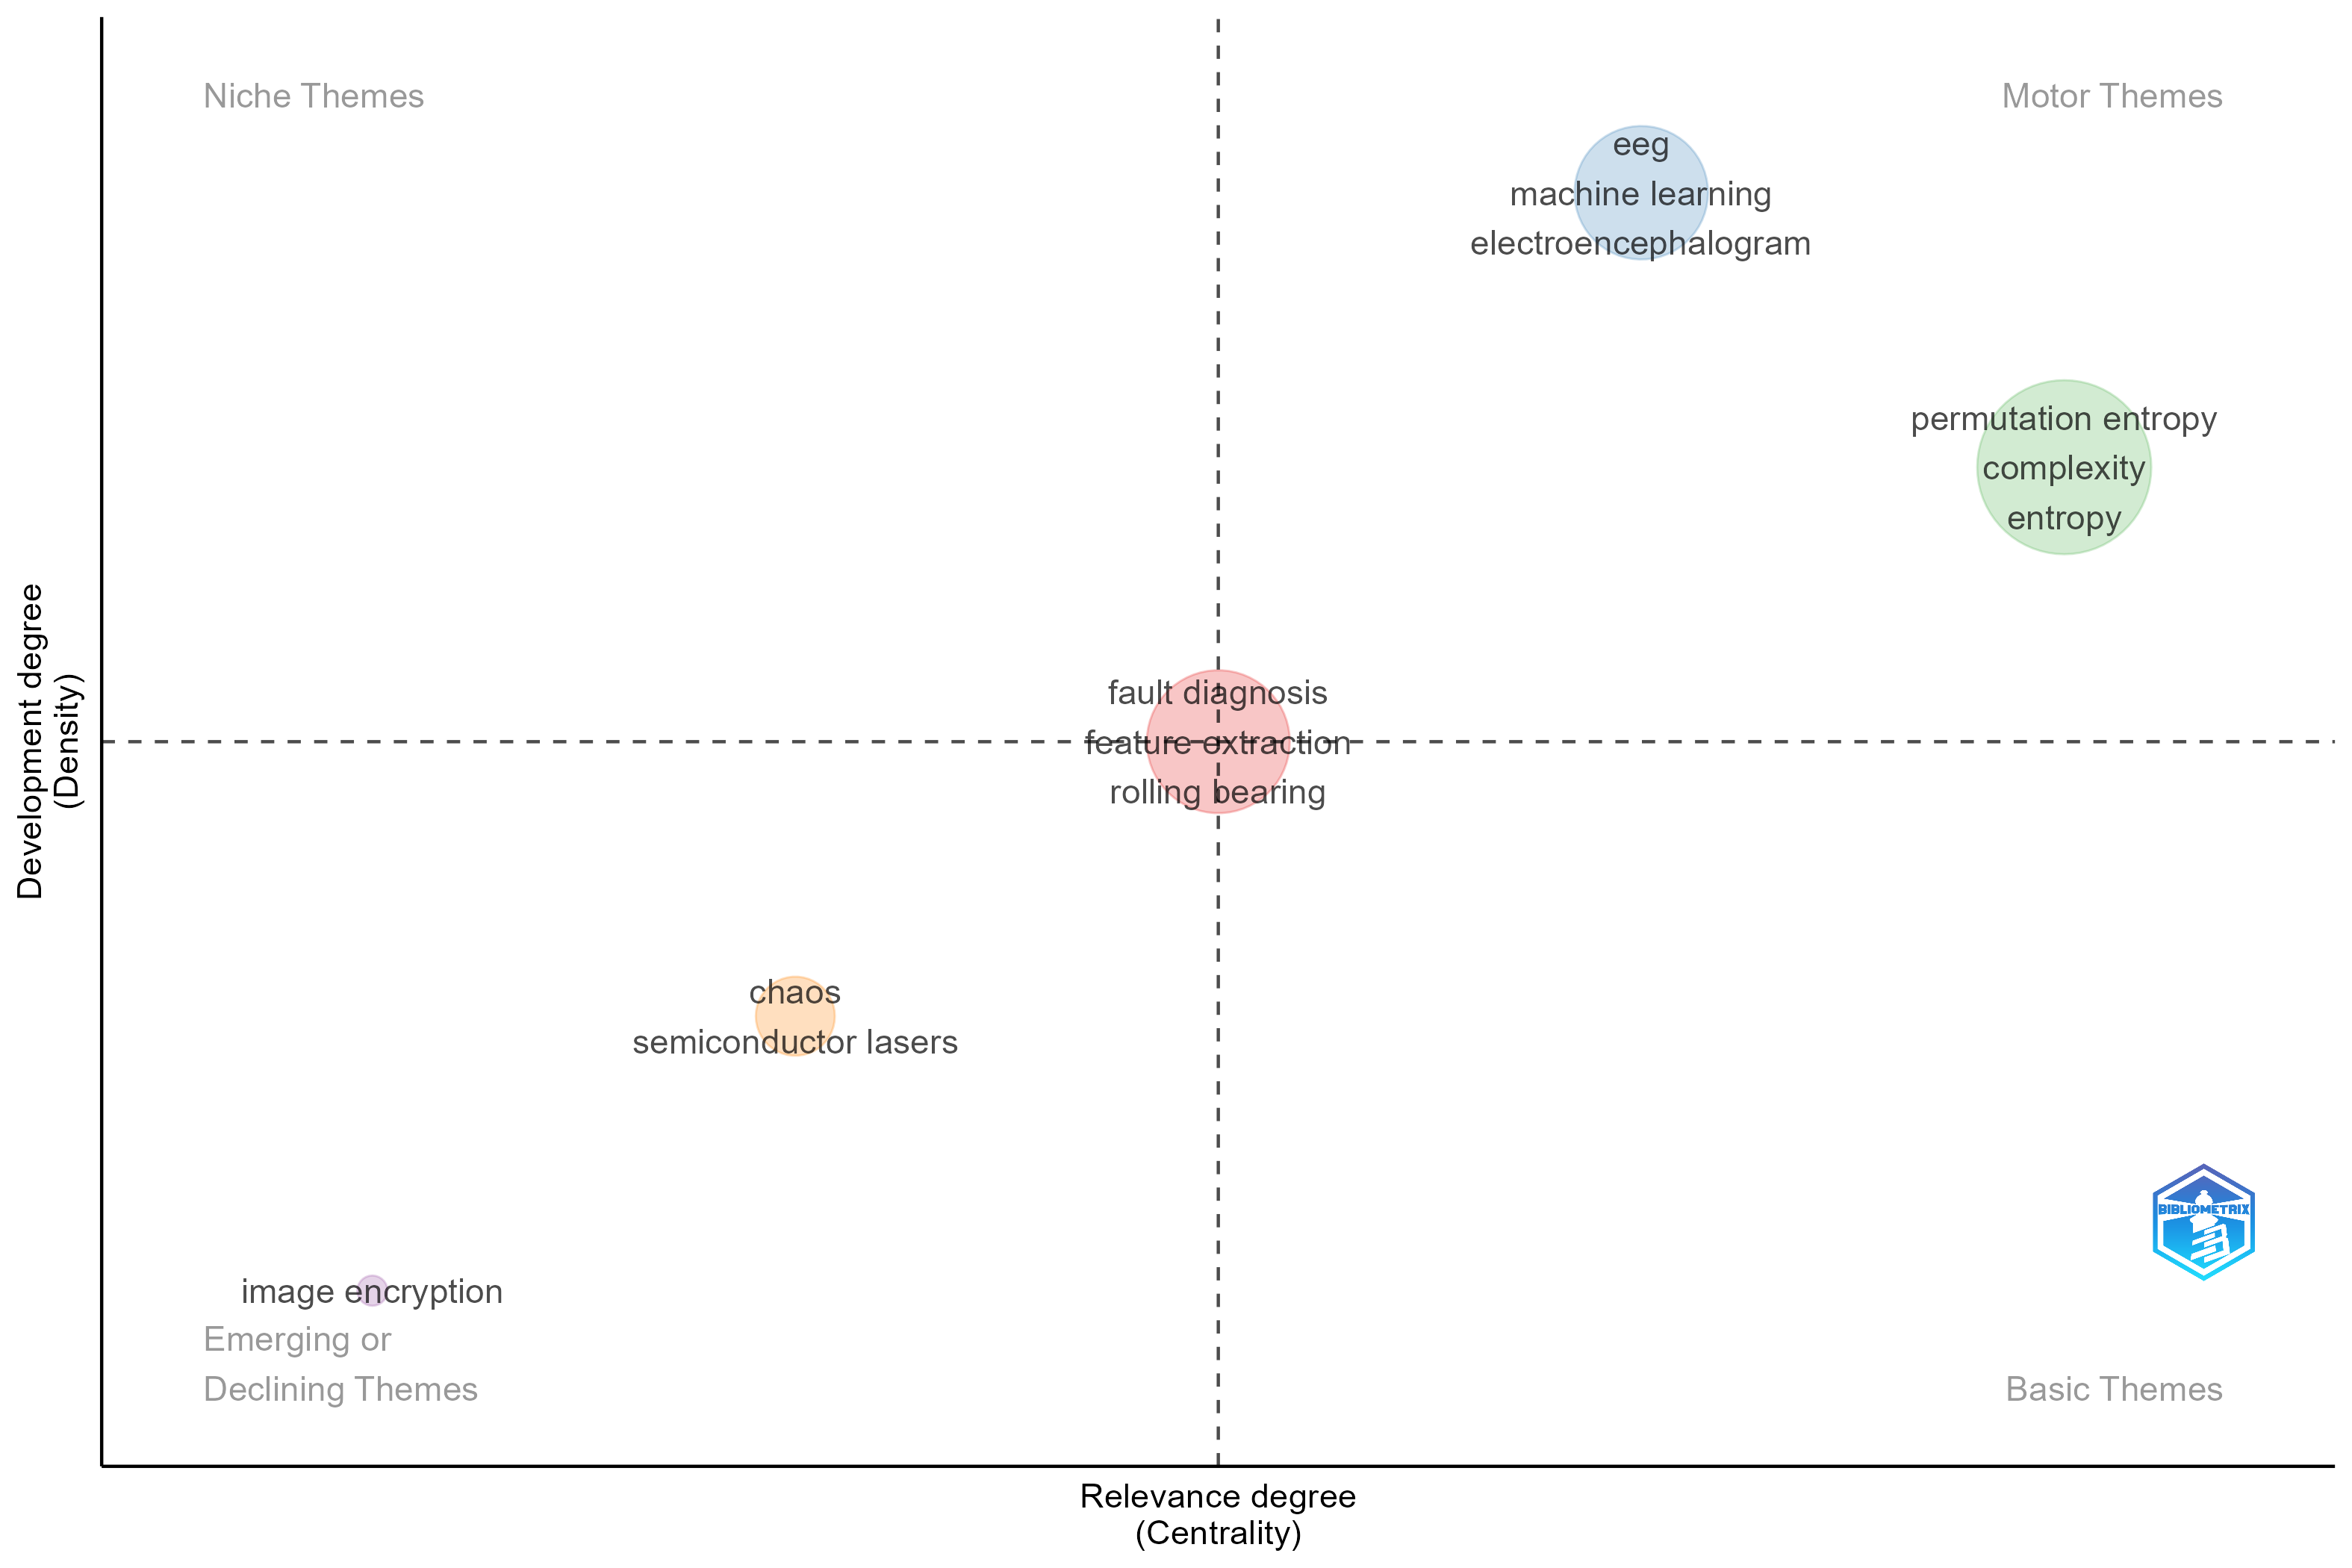
\includegraphics[width=\textwidth]{Figures/Chapter2/ThematicMap-2025-06-20}
	\caption{The Thematic Map generated by Bibliometrix.}
	\label{fig:ThematicMap}
\end{figure}

The map is divided into four quadrants based on two dimensions: centrality (relevance) and density (development). 
A right upper quadrant representing motor themes that are both well developed and highly interconnected areas of research, such as EEG, machine learning, permutation entropy, complexity, and other types of entropy. This theme is also at the core of current research, particularly in areas such as biomedical signal processing and nonlinear time series analysis. The consistent presence of entropy-based measures and machine learning highlights the interface between theory and practice.

Emerging or declining themes like image encryption reflect peripheral or potentially declining research interests, while chaos and semiconductor lasers hold theoretical interest, but its practical integration appears limited.  

A right down quadrant depicts basic themes indicates that opportunities for further theoretical and methodological advancement. 
Research fields such as fault diagnosis, feature extraction and rolling bearings are at the center of the map. Its moderate centrality and density mean that it is still active and is subject to evolving research fields. These topics are closely linked to engineering and diagnostic applications. These are important and growing areas which require further methodological refinement and integration.

The size of each circle further represents the frequency of the topic based on keyword occurrences associated with the publications. The clustering structure shows that entropy-related measures (such as the entropy of a permutation and the complexity of a system) are gaining ground not only in theory but also in practical applications such as EEG and machine learning.

From these results, we conclude that our research focus on entropy and complexity of permutation is relevant for many studies. These are basic concepts which are widely used in the literature, but which offer considerable potential for further development. Moreover, this thematic map shows that research is strongly focused on entropy-based methods, machine learning and biomedical applications, with fault diagnosis and feature extraction emerging as promising intermediate topics for further discuss.

\subsection{Factorial Analysis}
To identify the broad overview of the main research topics, we analyze the conceptual structure map. In this case we considered all keywords which are automatically generated by indexing databases. The shaded polygon in Figure~\ref{fig:factorialMap}  outlines the conceptual space defined by the most distinctive keywords. The X-axis (Dim 1) and the Y-axis (Dim 2) are the first two dimensions of the factorial space, and explain the largest differences in the co-occurrence of the keywords.

\begin{figure}[H]
	\centering
	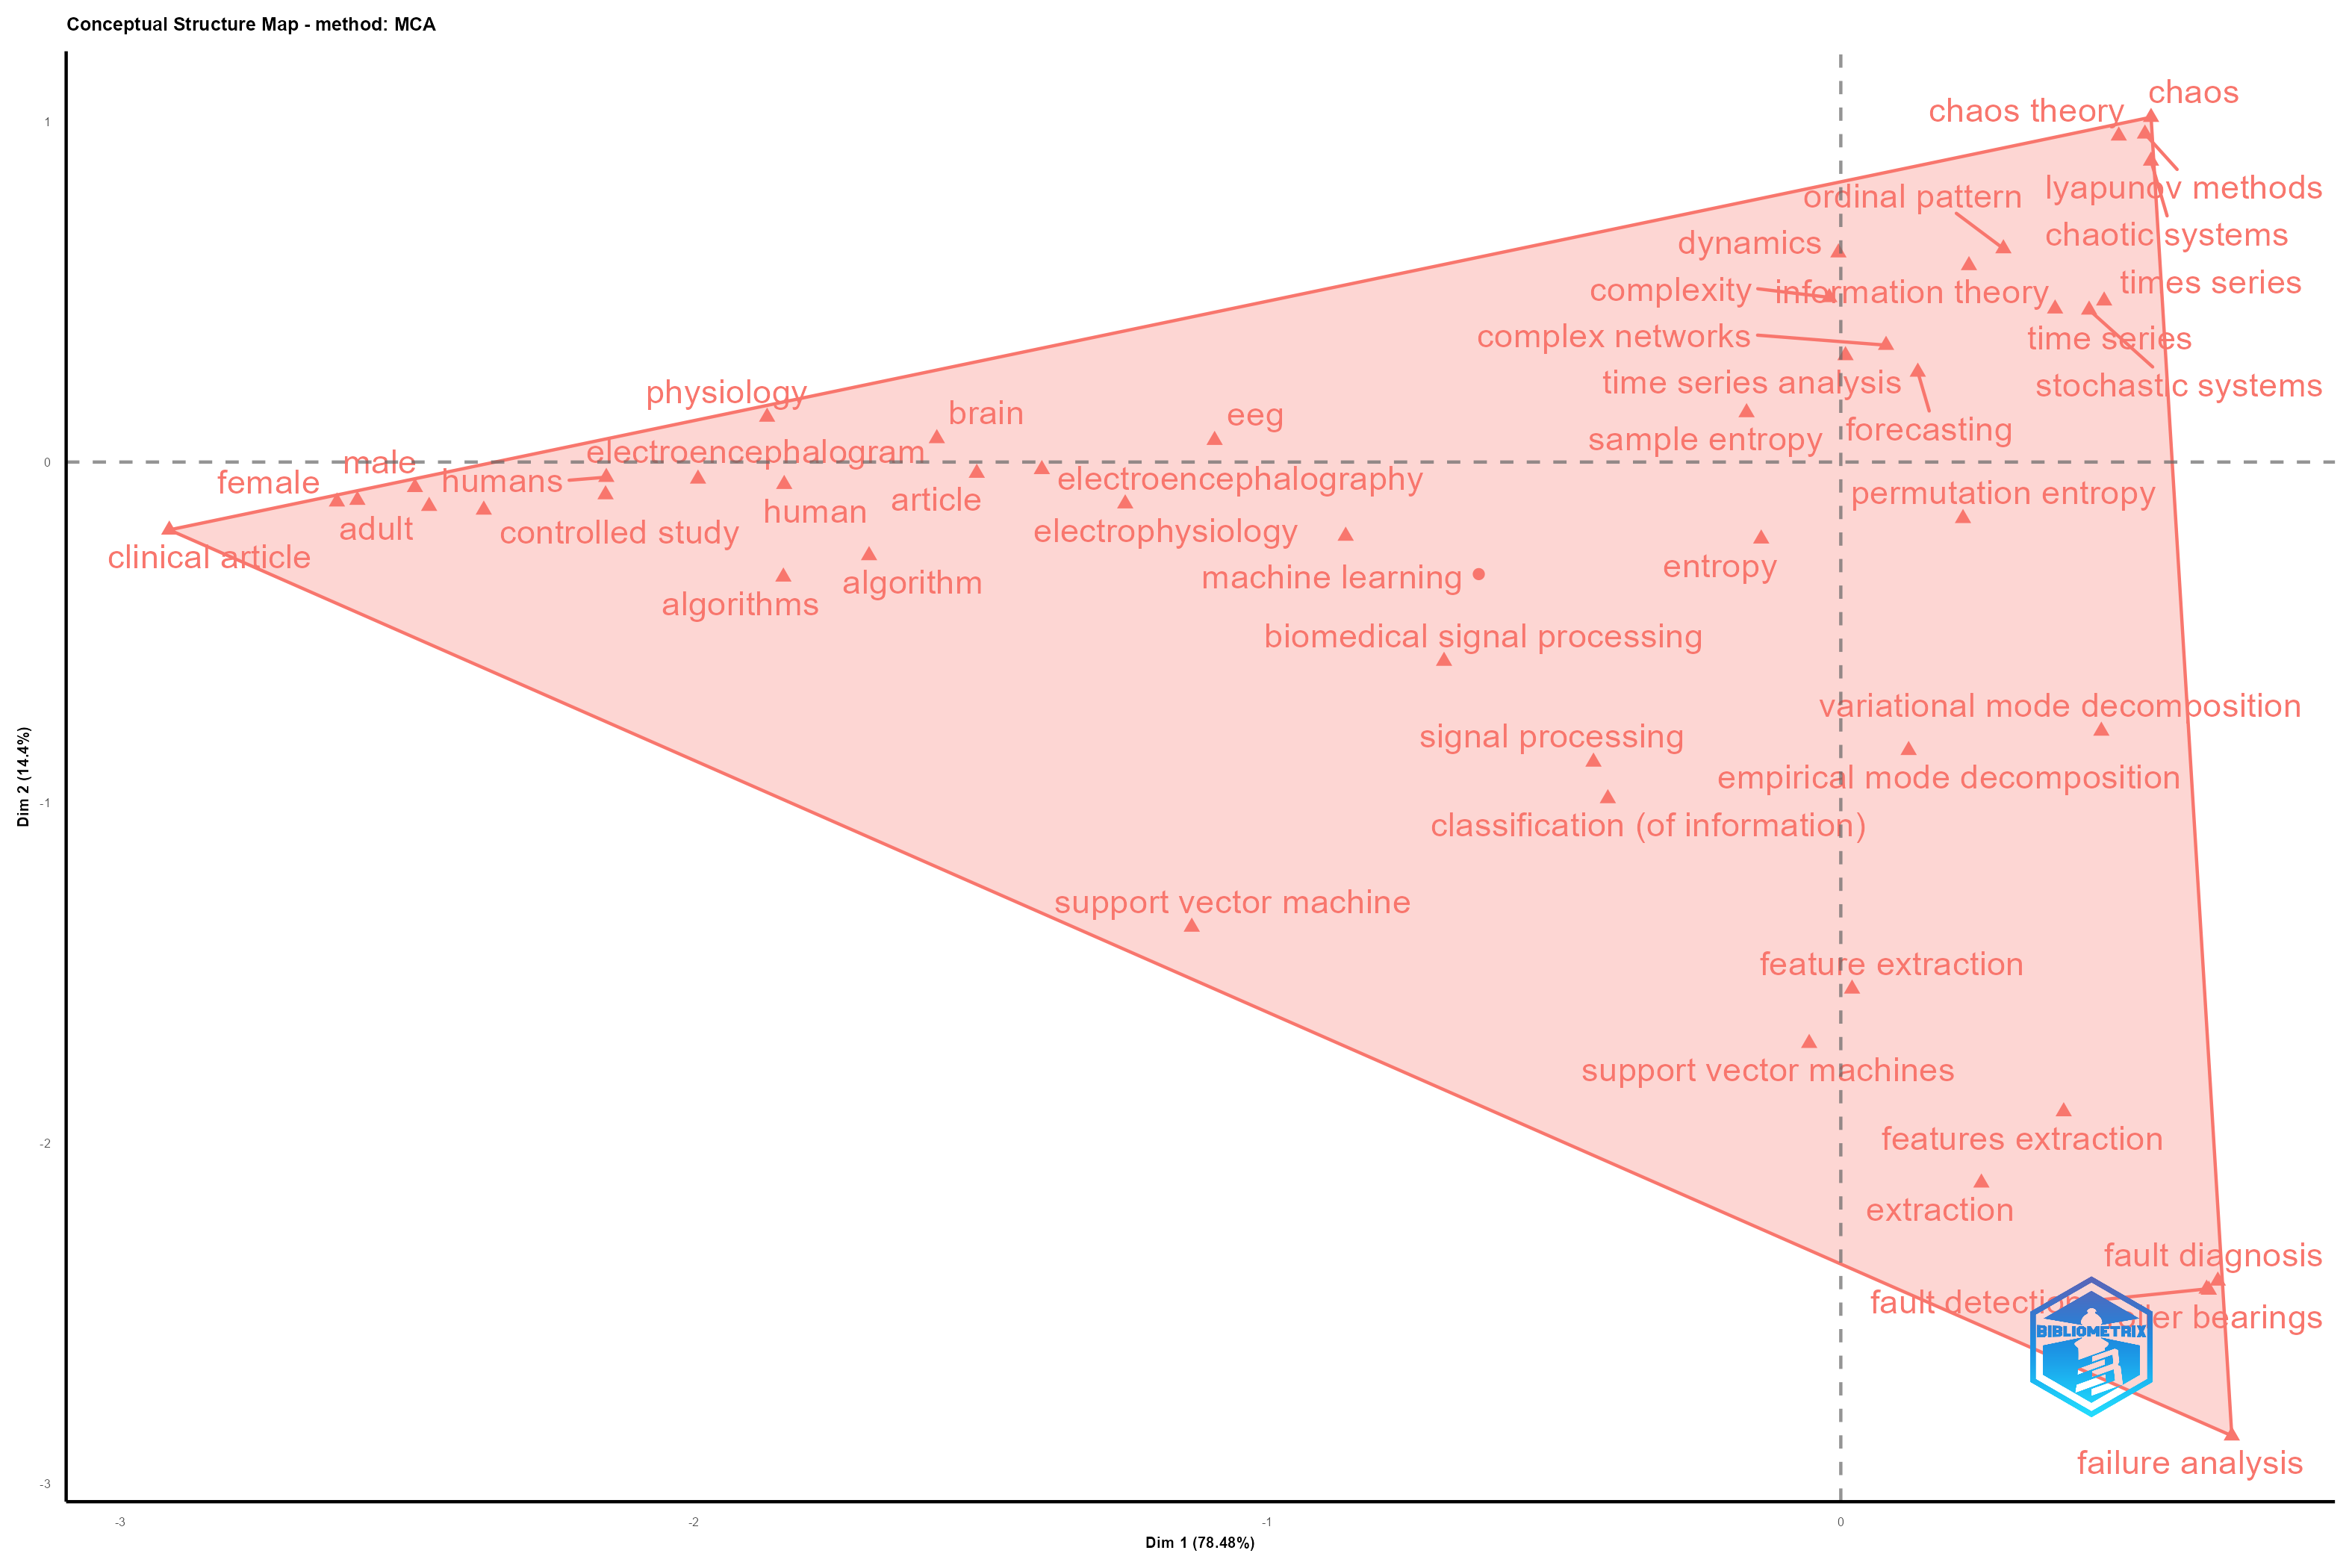
\includegraphics[width=0.9\textwidth]{Figures/Chapter2/FactorialMap}
	\caption{Conceptual Structure map generated by Bibliometrix.}
	\label{fig:factorialMap}
\end{figure}

The conceptual structure map reveals four major clusters:

The first cluster (upper right) includes theoretical concepts such as chaos theory, chaotic systems, Lyapunov methods, ordinal pattern, information theory, complex networks, and permutation entropy, forming the theoretical core of the research area.

The second cluster (lower right) includes practical applications such as feature extraction, empirical mode decomposition, variational mode decomposition, fault diagnosis, fault detection, and failure analysis, emphasizing the applied relevance of complexity-based time series analysis.

The third cluster (center) comprises terms related to biomedical signal processing and machine learning, including biomedical signal processing, EEG, support vector machine, classification, and machine learning, indicating the multidisciplinary applications of entropy measures.

A fourth, smaller cluster (left) includes clinical and physiological study keywords such as clinical article, controlled study, adult, male, female, humans, and physiology.

The conceptual map thus provides further evidence of the diverse applications and theoretical development surrounding ordinal patterns and complexity measures, supporting the originality and relevance of the present research.

\subsection{Conclusion and Justification of Research Focus}

Based on the thematic map and factorial analysis, research topics are categorized into four clusters and we will structure our review of the literature based on this clusters:

\begin{itemize}
	\item Permutation entropy, Complexity and other types of Entropy (section~\ref{Sec:ReviewTopicPE});
	\item EEG and Machine learning approach (section~\ref{Sec:ReviewTopicEEG});
	\item Fault diagnosis and failure analysis (section~\ref{Sec:ReviewTopicFault});
	\item Chaos other research works (section~\ref{Sec:ReviewTopicOthers});
	%\item Image encryption  (section~\ref{Sec:ReviewTopicImage}).
\end{itemize}

\section{Permutation entropy, Complexity and other types of Entropy}\label{Sec:ReviewTopicPE}
This cluster is associated with the keywords time series analysis, statistical complexity, nonlinear dynamics, ordinal patterns, entropy, and information theory. Although ordinal pattern based research have gained wide recognition as powerful tools for nonlinear time series analysis, with applications ranging from biomedical signal processing to cyber-physical systems, their theoretical and practical challenges remain unsolved \cite{Keller2017, Zanin2012}. 

Li et.al.~\cite{Li2015e} asses the complexity of short-term heartbeat interval series by using distribution entropy. They found that sample entropy (SampEn) or fuzzy entropy (FuzzyEn) quantifies essentially the randomness, which may not be uniformly identical to complexity. Zhang et.al.~\cite{Zhang2018d} uses the ordinal pattern technique to analyze dynamic behaviors such as regular, chaotic, or random patterns. The paper highlights the application of ordinal patterns in various fields, including ecology, finance, and physiology, where assessing variability and complexity is essential. It also emphasizes the advantages of using ordinal models to identify structural differences in time series that may not be detectable through traditional statistical methods.

Several studies have formalized the statistical behaviour of entropy and complexity measures derived from ordinal patterns, and have provided insights into their asymptotic distribution~\cite{Rey2024, Rey2023a} and sensitivity under the Multinomial law~\cite{Rey2023}. Despite these advances, the reliability of these measures in finite sampling conditions, in particular in non-stationary and noisy environments, remains limited~\cite{Borges2023}. 

Applications such as  Internet of Things(IoT) botnet detection~\cite{Borges2023} and  synthetic aperture radar(SAR) structure classification~\cite{Chagas2021a} have demonstrated the discriminability of ordinal-based features, particularly when combined with multiscale analysis; however, these methods often depend on the optimisation of parameters (dimension, delay) and may lack generalizability to a wide range of data. Similarly, the integration of entropy-complexity representations of class separation in time series dynamics~\cite{Borges2022}, although effective in a structured environment, poses problems when extended to real-time or data-scarce scenarios. 
%Data scarcity refers to the situation where there is insufficient data to meet the requirements of a system, particularly in enhancing the accuracy of predictive analytics.

The conceptual works linking ordinal complexity to broader ideas, such as the technological singularity~\cite{Modis2022} and the development of artistic expression ~\cite{Sigaki2018} illustrate the richness of the framework, but these studies are often qualitative and lack empirical rigour. 

Entropy-based clustering techniques have revealed evolving efficiency patterns in cryptocurrency markets~\cite{Sigaki2019}. The reliance on sensitive parameters and lack of standardized benchmarks highlight the need for more robust and interpretable methods to track market maturation reliably.

Moreover, white noise testing using entropy-complexity plane~\cite{Chagas2022a} and the use of ordinal properties in compressor signal diagnostics~\cite{Barbosa2024} demonstrate the methodological versatility of ordinal approaches. , the lack of uniform and reliable reference points prevents cross-domain comparison. Therefore, while ordinal methods provide a mathematically elegant and computationally efficient basis for obtaining information from complex signals, further research is needed to improve their statistical robustness, interpretability and adaptability to the challenges of the real world.

Although ordinal patterns are widely used in time series analysis, particularly in deriving entropy measures, studying their asymptotic distribution under the multinomial law, and analyzing the behavior of permutation entropy, their integration with confidence intervals remains widely unexplored. A systematic literature review reveals that while many studies investigate the statistical properties, asymptotic behavior, and robustness of ordinal pattern-based measures, no work has addressed the derivation or application of confidence intervals to assess the reliability or significance of time series clustering. This lack of statistical property limits interpretability and inference, especially when ordinal patterns are applied in data-driven algorithms. Therefore, this study aims to fill this gap by investigating how confidence intervals can be constructed for Shannon, Tsallis, and Renyi entropies, Fisher information measure, complexities, and how they may enhance time series clustering.

\section{EEG and Machine learning approach}\label{Sec:ReviewTopicEEG}

This cluster is based on multidisciplinary studies involving entropy measures applied to areas such as EEG, epilepsy, classification, heart rate variability, deep learning methods, and nonlinear analysis. An analysis of the author keywords indicates that many of these studies are centered on applications in biomedical signal processing. 

Acharya et al. ~\cite{Acharya2015a, Acharya2015, Acharya2017, Acharya2016, Acharya2019,  Acharya2017a, Acharya2018} have made significant contributions to biomedical signal processing by developing and evaluating advanced automated diagnostic tools across a wide range of clinical applications. Their work includes the use of entropy measures to detect epilepsy and heart disease from EEG and ECG signals, as well as the use of nonlinear dynamics to enhance the detection of sleep stages and the characterisation of focal EEG signals. In the cardiovascular field, they have performed comparative studies on the localization of myocardial infarction using various ECG leads and have developed empirical decomposition methods to identify congestive heart failure from cardiac signals. Another study by Lajnef et.al.~\cite{Lajnef2015} revealed that an automated approach to the classification of sleep stages using a multi-class support vector machine (SVM) based decision tree approach. The proposed method uses physiological signals (such as EEG, EOG, and EMG) to effectively classify the different stages of sleep.

\section{Fault diagnosis and failure analysis}\label{Sec:ReviewTopicFault}
This section primarily relates to the engineering applications of complexity-based time series analysis. The author keywords most commonly used to categorize this cluster include fault diagnosis, feature extraction, rolling bearing, support vector machine, variational mode decomposition, multiscale permutation entropy, dispersion entropy, rotating machinery, and empirical mode decomposition. 

Recent studies in bearing fault diagnosis often use entropy-based methods. Multiscale permutation entropy (MPE) and dispersion entropy are two popular techniques. These methods help detect complex changes in signals under different working conditions. For example, using variational mode decomposition with weighted entropy features helps extract useful information from non-stationary vibration signals. This improves how well faults can be classified~\cite{Lei2024a}. The weighted multiscale entropy method also works well by focusing on important frequency parts of the signal~\cite{Minhas2021a}. Self-adaptive hierarchical multiscale fuzzy entropy is also applied in bearing fault diagnosis. It makes fault detection easier without needing many manual settings~\cite{Yan2021}.  Composite multiscale fluctuation dispersion entropy can detect small fault signs even in noisy signals~\cite{Gan2019}. Some methods combine data decomposition with multiscale permutation entropy to better handle complex, changing systems~\cite{Yasir2018}. These improved entropy methods are also used in medical signal analysis, such as ECG or EEG, showing they work in other areas~\cite{Azami2017, HumeauHeurtier2015}. Dispersion entropy is known for being fast and good at finding small signal changes~\cite{Rostaghi2019,Rostaghi2016}, whereas multiscale permutation entropy still has issues. It can be affected by the length of the signal, noise, and it can be slow to compute~\cite{HumeauHeurtier2015, Zheng2014c}. Multiscale Permutation Entropy (MPE) with the Natural Visibility Graph (NVG) to enhance the fault diagnosis of rolling bearings by capturing both the dynamic complexity and structural features of time series method is proposed by Ma et.al.~\cite{Ma2025}. However, the method may still face limitations related to computational cost, parameter sensitivity, and the requirement for relatively long and noise-free signals to ensure reliable multiscale analysis.Therefore, more research is needed to make these methods faster, better with noise, and easier to use in different fault diagnosis tasks.

\section{Chaos and Other research works}\label{Sec:ReviewTopicOthers}
Research works related to chaos, semiconductor lasers, and image encryption are discussed in this category. 
A self-synchronous chaotic stream cipher, designed to resist active attacks and limit error propagation during image transmission, is a novel technique for image encryption.~\cite{Fan2018}. The 2D discrete wavelet transform, Arnold mapping, and a four-dimensional hyper-chaotic system with positive Lyapunov exponents are used to enhance the security and complexity of the encryption method. The advancement of chaos-based encryption and intelligent video security techniques in modern information systems has been demonstrated through a successful hardware implementation that transforms non-chaotic systems into chaotic ones, significantly enhancing unpredictability for secure communication. In addition, temporal action segmentation for video encryption has been analyzed to optimize computational resources and improve data protection~\cite{Gao2024,Liu2024k}

\section{Statistical Properties of Features from Ordinal Patterns}\label{Sec:StatisitcalProperty}

Although ordinal pattern based methods, such as permutation entropy, have been widely used for nonlinear time series analysis, the statistical properties of the features derived from these patterns, such as their distribution, variance, and confidence intervals remain under-explored and require further theoretical and empirical investigation. Therefore, based on the literature review we investigate the researchers who worked related to ordinal patterns, what kind of statistical properties of features used for their research work. Table~\ref{tab:StatisticalProperties} provides more information about the research articles and the test statistics or distributions they used.


\begin{longtable}{|p{5.5cm}|p{2.5cm}|p{6.5cm}|}
	\caption{The test statistics used by the research articles for hypothesis testing}
	\label{tab:StatisticalProperties} \\
	\hline
	\textbf{Paper Title/Reference} & \textbf{Distribution} & \textbf{Brief Description} \\
	\hline
	\endfirsthead
	
	\multicolumn{3}{c}%
	{{\bfseries \tablename\ \thetable{} -- continued from previous page}} \\
	\hline
	\textbf{Paper Title/Reference} & \textbf{Distribution} & \textbf{Brief Description} \\
	\hline
	\endhead
	
	\hline \multicolumn{3}{r}{{Continued on next page}} \\
	\endfoot
	
	\hline
	\endlastfoot
	
	A non-parametric independence test using permutation entropy. Matilla-García et.al.~\cite{MatillaGarcia2008} & Empirical (permutation) distribution & Tests independence by comparing the observed permutation entropy-based statistic to its distribution under random shuffling (permutation) of the time series.\\
	\hline
	Asymptotic distribution of certain types of entropy under the multinomial law. Rey at.at.~\cite{Rey2023} & Normal, Chi-squared ($\chi^2$) & Analyzes the asymptotic distribution (normal and chi-squared) of entropy estimators under the multinomial law. \\
	\hline
	Asymptotic distribution of entropies and Fisher information measure of ordinal patterns with applications. Reyet.al.~\cite{Rey2024} & Normal, Chi-squared ($\chi^2$) & Provides asymptotic distributions for entropy and Fisher information measures of ordinal patterns. \\
	\hline
	Asymptotic distribution of the permutation entropy. Rey at.al.~\cite{Rey2023a} & Normal & Derives the asymptotic normal distribution for permutation entropy estimators. \\
	\hline
	Asymptotic distribution of the statistical complexity under the multinomial law. Rey at.al.~\cite{Rey2025} & Normal, Chi-squared ($\chi^2$) & Studies the asymptotic distribution of statistical complexity measures derived from ordinal patterns under the multinomial law. \\
	\hline
	Assessing serial dependence in ordinal patterns processes using chi-squared tests with application to EEG data. Yamashita et.al.~\cite{YamashitaRiosDeSousa2022} & Chi-squared ($\chi^2$) & Applies chi-squared tests to assess serial dependence in ordinal pattern processes, with application to EEG data. \\
	\hline
	Bearing fault diagnosis based on Alpha-stable distribution feature extraction and SVM classifier. Chouri et.al.~\cite{Chouri2014} & Alpha-stable & Uses alpha-stable distribution parameters for feature extraction and SVM for classification in bearing fault diagnosis. \\
	\hline
	Belief permutation entropy of time series: A natural transition in analytical framework from probability theory to evidence theory. Xie et. al.~\cite{Xie2025} & Belief functions, Evidence theory basis & Introduces belief permutation entropy (BPE) using evidence theory (belief functions and mass assignments) and Deng entropy instead of classical probability distributions. \\
	\hline
	Markov modeling via ordinal partitions: An alternative paradigm for network-based time-series analysis. Sakellariou et.al.~\cite{Sakellariou2019} & Markov (transition) probabilities & Uses Markov models constructed from ordinal partitions to analyze time series as networks. \\
	\hline
	On the statistical properties of Multiscale Permutation Entropy: Characterization of the estimator's variance. Dávalos et.al.~\cite{Davalos2019a} & Normal (asymptotic) & Shows that the multiscale permutation entropy estimator is asymptotically normally distributed, allowing inference on variance.\\
	\hline
	Price predictability at ultra high frequency:Entropy based randomness test. Shternshis et.al.~\cite{Shternshis2025}& Chi-squared ($\chi^2$) & Proposes a randomness test for time series based on entropy, with asymptotic chi-squared distribution for the test statistic. \\
	\hline
	Statistical properties of the entropy from ordinal patterns. Chagas et.al.~\cite{Chagas2022} & Normal & Investigates statistical properties and asymptotic normality of entropy estimators from ordinal patterns. \\
	\hline
	The asymptotic distribution of the permutation entropy. Rey at.al.~\cite{Rey2023a} & Normal & Derives the asymptotic normal distribution for permutation entropy estimators. \\
	\hline
	The modified permutation entropy-based independence test of time series. Ashtari et.al.~\cite{AshtariNezhad2019} & Empirical (permutation) distribution & Tests independence by comparing the observed permutation entropy-based statistic to its distribution under random shuffling (permutation) of the time series.\\
	\hline
	White Noise Test from ordinal patterns in the entropy-complexity plane. Chagas et.al.~\cite{Chagas2022a} & Empirical Distribution & Used in white noise tests by repeatedly shuffling the time series to estimate the null distribution of the test statistic.\\
	\hline
	 Variance of entropy for testing time-varying regimes with an application to meme stocks Shternshis et.al.~\cite{Shternshis2024} & Chi-squared ($\chi^2$) & Introduces a rigorous hypothesis testing framework featuring an unbiased analytic approximation of sample Shannon entropy’s variance and an optimal rolling-window selection method.\\
	\hline
	
\end{longtable}










	% !TeX root = thesis.tex
\chapter{Methodology}\label{C:aim}

This chapter sets out the methodological framework used throughout the thesis. We begin by explaining why entropy and complexity measures are useful for time series analysis and what their limitations are (Section~\ref{Sec:AdvantagesLimitations}), and why the ordinal pattern approach of Bandt and Pompe is our representation of choice (Section~\ref{Sec:BP method}). Section~\ref{Sec:BackgroundKnowledge} defines the information-theoretic descriptors computed from ordinal pattern distributions: permutation entropy, disequilibrium, statistical complexity, the Rényi and Tsallis entropies, and the two forms of the Fisher information measure used in this work. Section~\ref{Sec:EntropyComplexity} describes the entropy--complexity plane. Section~\ref{Sec:AsymptoticDistribution} reviews the asymptotic distribution of these descriptors, which is what allows us to attach confidence intervals to them. Section~\ref{Sec:Software} describes the two R packages on which all computations rely, and Section~\ref{Subsec:GeneralFramework} summarises the general analysis procedure. Section~\ref{Sec:Simulation} describes the design of a simulation study in which time series with known generating mechanisms are used to test whether ordinal pattern features can separate different dynamics, and Section~\ref{Sec:Clustering} presents the clustering and classification methods used in this study and in the applications. Finally, Section~\ref{Sec:Applications} explains how the same framework is applied to the two geophysical problems studied in this thesis: Synthetic Aperture Radar (SAR) time series for land cover classification and seismic amplitude data from Whakaari/White Island.

\section{Entropy and Complexity Analysis in Time Series: Advantages and Limitations}\label{Sec:AdvantagesLimitations}

Many systems of scientific interest evolve over time in ways that are neither perfectly regular nor purely random. Entropy and complexity measures give us a way to describe where a system sits between these two extremes. Shannon entropy quantifies the uncertainty of a probability distribution. Permutation entropy applies the same idea to the distribution of ordinal patterns extracted from a time series, so that it measures how diverse the order structure of the series is, rather than how spread out its values are.

Entropy on its own, however, cannot tell a structured system apart from a noisy one when both have similar entropy values. Statistical complexity was introduced to fill this gap: it combines entropy with a measure of how far the distribution is from uniform distribution, and so describes the balance between order and disorder. Used together, entropy and complexity are well suited to nonlinear dynamics, that is, systems in which outputs are not proportional to inputs and where small changes can have large or unpredictable effects. Such behaviour is common in biological, financial, climate and geophysical systems.

These measures do have practical limitations. Their values depend on the choice of parameters, in particular the embedding dimension and the time delay. They require enough data for the empirical pattern distribution to be a reliable estimate of the underlying one, and the data often need some preprocessing. Interpretation also requires knowledge of the application domain; a high entropy value is not informative unless one knows what a high value means for the system under study.

Despite these limitations, entropy and complexity measures remain valuable. Classical linear tools such as the autocorrelation function, regression and Fourier analysis assume proportional relationships and, in most cases, stationarity. Entropy and complexity measures make no such assumptions, and they are designed to respond to irregularity, changes in pattern and chaotic behaviour. This is precisely the kind of behaviour we expect in the remote sensing and volcanic data analysed later in this thesis.

\section{The Bandt and Pompe Method: A Robust Approach} \label{Sec:BP method}

Classical estimators of complexity, such as the correlation dimension~\cite{Grassberger1983}, fractal dimension and Lyapunov exponents~\cite{Wolf1985}, were developed for low-dimensional dynamical systems~\cite{Huffaker2018}. These are systems whose behaviour can be described by a small number of variables or equations, typically two or three, such as the logistic map or a simple pendulum. Although their dynamics can be rich and even chaotic, their structure is relatively easy to recover from data. The Lyapunov exponent, for example, measures the average rate at which nearby trajectories diverge or converge, and is a natural indicator of chaos in this setting. In real data, however, these estimators tend to perform poorly: they need long and clean records, and their estimates deteriorate quickly once noise is present~\cite{PhysRevLett.88.174102,Huffaker2018}.

Bandt and Pompe~\cite{PhysRevLett.88.174102} proposed a different route. Instead of working with the values of the series, they replace each short window of consecutive observations by its ordinal pattern, that is, the permutation that sorts the values in the window. The time series is thereby turned into a sequence of symbols, and all subsequent analysis is carried out on the distribution of these symbols. The main advantages of this approach are the following:
\begin{itemize}
	\item it is conceptually simple and requires no model of the data;
	\item it is computationally fast, even for very long series;
	\item it is robust to noise and to outliers, because small perturbations rarely change the order of values in a window;
	\item it is invariant under strictly increasing (monotonic) transformations of the data, so that, for instance, working with amplitudes or with their logarithms (decibels) yields the same patterns.
\end{itemize}
Because ordinal patterns are built from consecutive observations, the method also respects the temporal (causal) order of the data. These properties explain why it has been used so widely to distinguish chaotic from stochastic signals.

The method also has known shortcomings. Information about amplitude is discarded, ties between equal values must be resolved by some convention, and the number of possible patterns, $D!$, grows very quickly with the embedding dimension $D$, which increases the amount of data required. Several extensions of the original method have been proposed to address these issues. In this thesis we use the original formulation with time delay $\tau=1$ and choose $D$ so that the length of each series is large relative to $D!$.

\section{Information-Theoretic Descriptors of Ordinal Patterns} \label{Sec:BackgroundKnowledge}

Bandt and Pompe computed the Shannon entropy of the histogram of ordinal patterns and used it, among other applications, to detect chaotic components in time series. Rosso et al.~\cite{EEGAnalysisUsingWaveletBasedInformationTools} extended this analysis by adding a second dimension: the statistical complexity computed from the same histogram. Plotting one quantity against the other gives the entropy--complexity plane, which has since been used to visualise and characterise dynamical regimes as system parameters change~\cite{Bandt2005,Cao2004,DeMicco2012a,Kowalski2007,Kowalski2011b,Rosso2010a,Zunino2010a,Zunino2012a}, and has been applied to optical chaos~\cite{Liu2016f,Soriano2011a,Toomey2014,Yang2015e,Zunino2011a}, hydrology~\cite{Lange2013,Serinaldi2014,Stosic2016}, geophysics~\cite{Consolini2014,Saco2010,Sippel2016}, engineering~\cite{Aquino2017,Aquino2015,Redelico2017a,Yan2012}, biometrics~\cite{Rosso2016}, the assessment of pseudo-random number generators~\cite{DeMicco2008,DeMicco2009}, biomedical signal analysis~\cite{Li2014b,Li2008b,Li2007,Liang2015b,Montani2015a,Montani2014,Montani2014a,Montani2015,Morabito2012,Parlitz2012,Perinelli2025,Perinelli2019,Zanin2012}, and econophysics~\cite{Bariviera2015a,Bariviera2015,Bariviera2016,Zanin2012,Zunino2016a,Zunino2009,Zunino2010}, among other fields.

Closer to the problems studied in this thesis, information-theoretic descriptors have been used to track volcanic and hydrothermal activity, with permutation entropy anticipating eruptions of the Strokkur geyser~\cite{Sudibyo2022} and amplitude-based Fisher--Shannon and Shannon entropy measures revealing changes before eruptions at El Hierro and Volcán de Colima~\cite{Telesca2014,ReyDevesa2023}.
%Further in remote sensing, ordinal pattern features of Sentinel-1 SAR time series have been shown to discriminate between land cover classes~\cite{Dilhani2026SAR}.

\subsection{Notation}\label{Subsec:Notation}

We use the following notation throughout the thesis. Let $\mathbf{x}=(x_1,x_2,\dots,x_{n+D-1})$ be a real-valued time series and $D\geq 2$ the embedding dimension. For $t=1,\dots,n$ we form the overlapping windows $\mathbf{s}_t=(x_t,x_{t+1},\dots,x_{t+D-1})$ and assign to each window its ordinal pattern, as described in Chapter~\ref{C:intro}. There are $k=D!$ possible patterns, which we denote by $\pi^1,\pi^2,\dots,\pi^k$. Let $N_\ell$ be the number of windows whose pattern is $\pi^\ell$. The empirical probability function of ordinal patterns is then
\begin{equation}
	\widehat{\mathbf{p}}=\left(\frac{N_1}{n},\frac{N_2}{n},\dots,\frac{N_k}{n}\right)=(\widehat{p}_1,\widehat{p}_2,\dots,\widehat{p}_k),
	\label{eq:EmpiricalP}
\end{equation}
which estimates the true (unknown) probability function $\mathbf{p}=(p_1,\dots,p_k)$. All descriptors below are written for a generic probability function $\mathbf{p}$; in practice they are evaluated at $\widehat{\mathbf{p}}$. Throughout, $\log$ denotes the natural logarithm and we adopt the convention $0\log 0=0$.

\subsection{Permutation entropy}

The Shannon entropy of $\mathbf{p}$ is
\begin{equation}
	S(\mathbf{p})=-\sum_{\ell=1}^{k}p_\ell\log p_\ell ,
	\label{eq:ShannonUnnorm}
\end{equation}
and its normalised version,
\begin{equation}
	H(\mathbf{p})=\frac{S(\mathbf{p})}{\log k}=-\frac{1}{\log k}\sum_{\ell=1}^{k}p_\ell\log p_\ell ,
	\label{eq:NormShannon}
\end{equation}
is known as the permutation entropy when $\mathbf{p}$ is an ordinal pattern distribution. The normalisation keeps the entropy in the unit interval, which allows comparisons across embedding dimensions:
\begin{itemize}
	\item $H(\mathbf{p})=0$ when a single pattern occurs, i.e., $p_\ell=1$ for some $\ell$;
	\item $H(\mathbf{p})=1$ when all patterns are equally likely, i.e., $p_\ell=1/k$ for every $\ell$.
\end{itemize}
Low values therefore indicate regular, predictable dynamics, while values close to one indicate that the order structure is close to random.

\subsection{Disequilibrium and statistical complexity}

Permutation entropy measures disorder, but it cannot fully characterise the dynamics: quite different processes can have similar entropy. López-Ruiz et al.~\cite{lopez1995statistical} addressed this by introducing the disequilibrium $Q$, which measures how far $\mathbf{p}$ is from the uniform, non-informative distribution $\mathbf{u}=(1/k,\dots,1/k)$. In their original proposal the distance was Euclidean. Lamberti et al.~\cite{lamberti2004intensive} replaced it with the Jensen--Shannon divergence, which is symmetric, bounded, and has a clear information-theoretic meaning:
\begin{equation}
	J(\mathbf{p},\mathbf{u})=S\!\left(\frac{\mathbf{p}+\mathbf{u}}{2}\right)-\frac{1}{2}S(\mathbf{p})-\frac{1}{2}S(\mathbf{u}),
	\label{eq:JSD}
\end{equation}
where $S(\mathbf{u})=\log k$. The divergence attains its maximum when all the probability is concentrated on a single pattern, in which case
\begin{equation}
	J_{\max}=-\frac{1}{2}\left[\frac{k+1}{k}\log(k+1)-2\log(2k)+\log k\right].
	\label{eq:JSDmax}
\end{equation}
The normalised disequilibrium is
\begin{equation}
	Q(\mathbf{p})=\frac{J(\mathbf{p},\mathbf{u})}{J_{\max}},
	\label{eq:Disequilibrium}
\end{equation}
which equals zero for the uniform distribution and one for a degenerate distribution. Following Lamberti et al.~\cite{lamberti2004intensive}, the statistical complexity is the product
\begin{equation}
	C(\mathbf{p})=H(\mathbf{p})\,Q(\mathbf{p}).
	\label{eq:Complexity}
\end{equation}
Since both factors lie in $[0,1]$, so does $C$. The product form means that complexity is small at both extremes, perfect order ($H=0$) and complete randomness ($Q=0$), and is largest for distributions that combine moderate disorder with marked structure. To make clear which information measure it is built on, we also write $C_S=HQ$ and call it the Shannon complexity.

\subsection{Rényi and Tsallis entropies}

Shannon entropy weights every pattern by its probability. Generalised entropies introduce a parameter $q$ that changes this weighting, giving more or less importance to rare patterns. The Rényi entropy~\cite{renyi1961measures} is
\begin{equation}
	H_{R}^{q}(\mathbf{p})=\frac{1}{1-q}\log\sum_{\ell=1}^{k}p_\ell^{\,q},\qquad q\in\mathbb{R}^{+}\setminus\{1\},
	\label{eq:Renyi}
\end{equation}
and the Tsallis entropy~\cite{tsallis1988possible} is
\begin{equation}
	H_{T}^{q}(\mathbf{p})=\sum_{\ell=1}^{k}\frac{p_\ell-p_\ell^{\,q}}{q-1},\qquad q\in\mathbb{R}\setminus\{1\}.
	\label{eq:Tsallis}
\end{equation}
Both reduce to the Shannon entropy~\eqref{eq:ShannonUnnorm} in the limit $q\to1$. Values $q<1$ emphasise rare patterns and values $q>1$ emphasise dominant ones. In our applications we use $q=1.5$, in line with the value used by Rey et al.~\cite{Rey2023}.

As with the Shannon entropy, both quantities are normalised by their value under the uniform distribution, which is their maximum:
\begin{equation}
	\widetilde{H}_{R}^{q}(\mathbf{p})=\frac{H_{R}^{q}(\mathbf{p})}{\log k},
	\qquad
	\widetilde{H}_{T}^{q}(\mathbf{p})=\frac{(q-1)\,H_{T}^{q}(\mathbf{p})}{1-k^{1-q}},
	\label{eq:NormRenyiTsallis}
\end{equation}
so that both lie in $[0,1]$. Replacing $H$ by $\widetilde{H}_{R}^{q}$ or $\widetilde{H}_{T}^{q}$ in~\eqref{eq:Complexity}, while keeping the same disequilibrium $Q$, gives the Rényi complexity $C_R=\widetilde{H}_{R}^{q}\,Q$ and the Tsallis complexity $C_T=\widetilde{H}_{T}^{q}\,Q$.

\subsection{Fisher information measure}\label{Subsec:Fisher}

The Fisher information~\cite{frieden2004science} was originally defined for continuous densities as the expected squared derivative of the log-density. It therefore measures how sharply a distribution changes, rather than how spread out it is. This makes it a local measure, in contrast with Shannon entropy, which is global: entropy is unchanged by any reordering of the probabilities, whereas the Fisher information responds to differences between neighbouring probabilities. As a consequence, it is more sensitive to small changes and perturbations in the pattern distribution.

For a discrete distribution, the derivative is replaced by differences between consecutive probabilities. Two discretisations appear in the literature, and both are used in this thesis.

\paragraph{Form 1: square-root (Hellinger-type) discretisation.} Following Sánchez-Moreno et al.~\cite{sanchez2009discrete}, the first form is
\begin{equation}
	F_1(\mathbf{p})=F_0\sum_{\ell=1}^{k-1}\left(\sqrt{p_{\ell+1}}-\sqrt{p_\ell}\right)^2,
	\label{eq:Fisher1}
\end{equation}
where $F_0$ is a normalisation constant. In this thesis we use $F_0=4$, the constant adopted by Rey et al.~\cite{Rey2024} in their derivation of the asymptotic distribution of the Fisher information of ordinal patterns. Working with square roots of probabilities avoids divisions by zero when some patterns are not observed, and it is the form for which asymptotic results are available (Section~\ref{Subsec:OtherAsymptotics}).

\paragraph{Form 2: difference-ratio discretisation.} The second form, proposed by Ferri et al.~\cite{Ferri2009} and used in our study of SAR land cover, is
\begin{equation}
	F_2(\mathbf{p})=\frac{1}{4}\sum_{\ell=1}^{k-1}\frac{2\,(p_{\ell+1}-p_\ell)^2}{p_{\ell+1}+p_\ell}
	=\frac{1}{2}\sum_{\ell=1}^{k-1}\frac{(p_{\ell+1}-p_\ell)^2}{p_{\ell+1}+p_\ell},
	\label{eq:Fisher2}
\end{equation}
where terms with $p_{\ell+1}+p_\ell=0$ are taken as zero. In the implementation, a small constant ($10^{-12}$) is added to the denominator to avoid numerical division by zero.

\paragraph{Relation between the two forms.} The two forms are closely related. Since $(\sqrt{a}-\sqrt{b})^2=(a-b)^2/(\sqrt{a}+\sqrt{b})^2$, and $a+b\leq(\sqrt{a}+\sqrt{b})^2\leq 2(a+b)$ for $a,b\geq 0$, each term of~\eqref{eq:Fisher1} lies between one half and one times the corresponding term of $\sum (p_{\ell+1}-p_\ell)^2/(p_{\ell+1}+p_\ell)$. Hence
\begin{equation}
	F_2(\mathbf{p})\;\leq\;\frac{F_1(\mathbf{p})}{F_0}\;\leq\;2\,F_2(\mathbf{p}).
	\label{eq:FisherBounds}
\end{equation}
The two measures therefore carry essentially the same information about local changes in the distribution, but they are on different scales and are not interchangeable. For this reason we always state which form is being used, and we never compare numerical values of $F_1$ with values of $F_2$.

A feature shared by both forms is that, unlike the entropies, they depend on the order in which the $k$ patterns are listed. Olivares et al.~\cite{Olivares2012b} discussed this ambiguity and showed that different ordering schemes can lead to different values. The ordering is fixed by the software used to enumerate the patterns, and we keep the same ordering within each analysis so that results are comparable.

\paragraph{Fisher complexity.} By analogy with~\eqref{eq:Complexity}, we define the Fisher complexity as
\begin{equation}
	C_F(\mathbf{p})=F(\mathbf{p})\,Q(\mathbf{p}),
	\label{eq:FisherComplexity}
\end{equation}
where $F$ is whichever Fisher form is used in the analysis at hand. Plotting $C_F$ against $F$ gives the Fisher information--complexity plane, which we use alongside the entropy--complexity plane.

\section{The Entropy--Complexity Plane} \label{Sec:EntropyComplexity}

The entropy--complexity plane, also written $H\times C$, is a two-dimensional representation in which each time series is placed according to the permutation entropy and statistical complexity of its ordinal pattern distribution. For a given embedding dimension $D$, not every point of the unit square can be reached, and the location of a series within the feasible region says a great deal about its dynamics.

\subsection{Key dynamics in the plane}

Two extreme cases help to read the plane.
\begin{enumerate}
	\item \textbf{Highly ordered systems}, whose behaviour is predictable and often repeats regularly. A strictly monotonic series, for example, produces a single ordinal pattern. Its entropy is $H=0$, its disequilibrium is maximal ($Q=1$), and so its complexity is $C=0$. It is mapped to the point $(0,0)$.
	\item \textbf{Completely random systems}. White noise produces all patterns with equal probability, so that $H=1$ and the disequilibrium vanishes ($Q=0$). It is mapped to the point $(1,0)$: maximal entropy and no structure.
\end{enumerate}
The existence of these extreme values was established by Anteneodo and Plastino~\cite{anteneodo1996some}. Between them, deterministic chaotic systems tend to occupy the upper part of the region, with intermediate entropy and high complexity, whereas correlated stochastic processes lie closer to the lower boundary.

Martin et al.~\cite{Martin2006} derived the boundaries of the feasible region using geometrical arguments in the space of probability functions. The lower boundary is a smooth curve, whereas the upper boundary consists of $D!-1$ separate segments; as $D$ increases, the upper boundary approaches a smooth curve. Figure~\ref{fig:complexity} shows the feasible region for embedding dimensions $3$ to $6$. Figure~\ref{fig:tentimeseries} shows ten time series together with their positions in the $H\times C$ plane for $D=6$.

\begin{figure}[H]
	\centering
	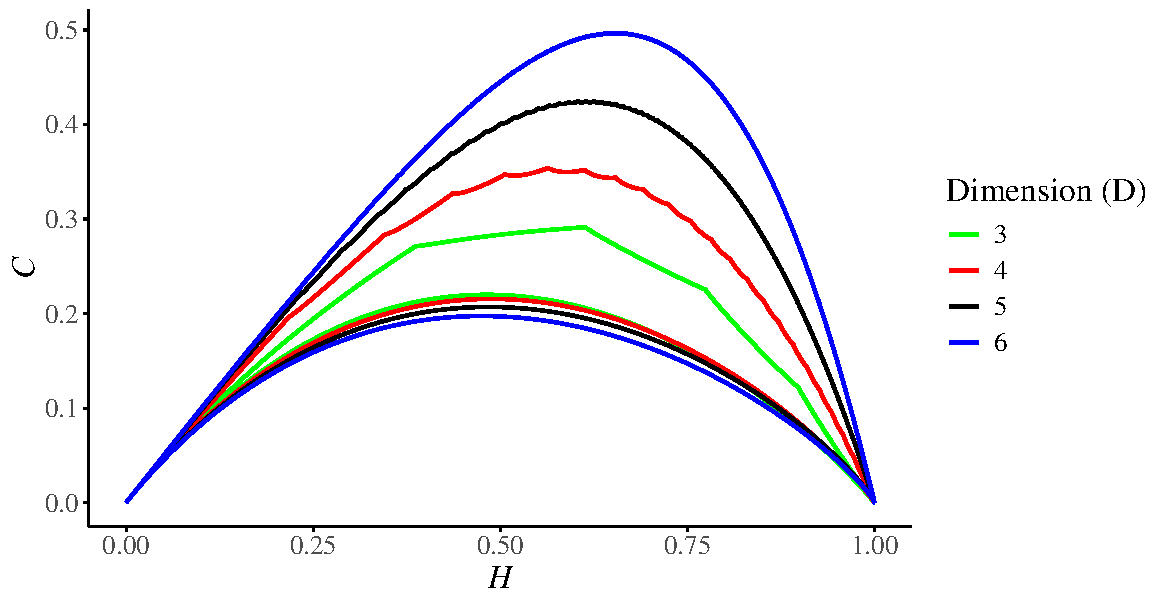
\includegraphics[width=0.7\textwidth]{Figures/Chapter3/complexity plane}
	\caption{Feasible region of the entropy--complexity plane for embedding dimensions $D=3,4,5$ and $6$.}
	\label{fig:complexity}
\end{figure}

\begin{figure}[H]
	\centering
	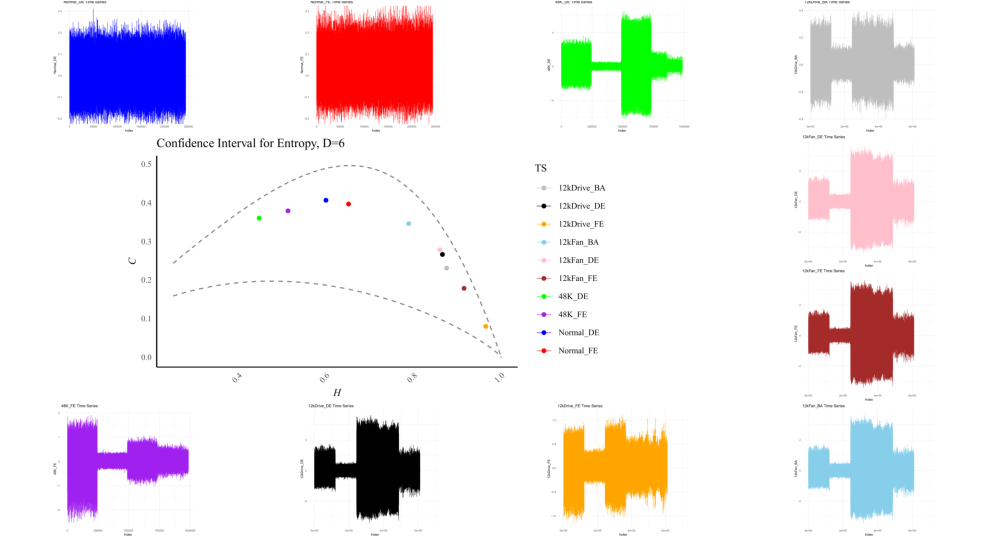
\includegraphics[width=0.7\textwidth]{Figures/Chapter3/combined plot}
	\caption{Ten time series and their positions in the $H\times C$ plane for embedding dimension $D=6$.}
	\label{fig:tentimeseries}
\end{figure}

Unlike the entropy--complexity plane, the Fisher information--complexity plane has no known closed-form boundaries, so we use it as a descriptive tool rather than one with a fixed reference frame.

\section{Asymptotic Distribution of Ordinal Pattern Descriptors}\label{Sec:AsymptoticDistribution}

Every descriptor in Section~\ref{Sec:BackgroundKnowledge} is computed from the estimate $\widehat{\mathbf{p}}$ and is therefore a random quantity. Two series may produce different entropy values simply because of sampling variability, so to compare series in a meaningful way we need to know how much these descriptors vary. The exact distribution of these statistics is difficult to obtain, and the literature has approached the problem in two ways.

The first approach is empirical. Here one simulates or resamples many series from a model and builds the distribution of the descriptors directly from the resulting values. Combined with knowledge of the expected variability of entropy and complexity, this allows hypothesis tests for a wide range of models~\cite{Chagas2022a,DeMicco2008,Larrondo2005,Larrondo2006}. Its drawback is that it requires a model and can be computationally expensive.

The second approach, which we follow, is asymptotic. It gives closed-form approximations of the variance that hold when the number of patterns $n$ is large. Two models are considered. In the \emph{multinomial model}, the patterns are treated as independent draws from $\mathbf{p}$. This is a convenient simplification, but it is not strictly true: consecutive windows overlap in $D-1$ observations, so neighbouring patterns are dependent. The second model accounts for this \emph{serial dependence}.

\subsection{Asymptotic distribution of the Shannon entropy under the multinomial model}\label{Subsec:Multinomial}

Under the multinomial model, the vector of counts $\mathbf{N}=(N_1,\dots,N_k)$, with $\sum_{\ell}N_\ell=n$, follows a multinomial distribution $\mathbf{N}\sim\mathrm{Mult}(n,\mathbf{p})$ with probability mass function
\[
\Pr(\mathbf{N}=\mathbf{m})=n!\prod_{\ell=1}^{k}\frac{p_\ell^{m_\ell}}{m_\ell!},
\]
and moments
\[
\mathrm{E}(N_\ell)=np_\ell,\qquad
\mathrm{Var}(N_\ell)=np_\ell(1-p_\ell),\qquad
\mathrm{Cov}(N_\ell,N_j)=-np_\ell p_j \quad (\ell\neq j).
\]
The maximum likelihood estimator of $p_\ell$ is $\widehat{p}_\ell=N_\ell/n$, which is exactly~\eqref{eq:EmpiricalP}. By the invariance property of maximum likelihood estimators, $g(\widehat{\mathbf{p}})$ is the maximum likelihood estimator of $g(\mathbf{p})$ for any function $g$; in particular, $S(\widehat{\mathbf{p}})$ estimates $S(\mathbf{p})$. Written in terms of the counts,
\begin{align}
	S(\widehat{\mathbf{p}})
	&=-\sum_{\ell=1}^{k}\frac{N_\ell}{n}\log\frac{N_\ell}{n}
	=\log n-\frac{1}{n}\sum_{\ell=1}^{k}N_\ell\log N_\ell .
	\label{eq:AsymEntropy}
\end{align}
The unnormalised entropy lies between $0$ and $\log k$; the minimum is attained when $p_\ell=1$ for some $\ell$ and $p_j=0$ for all $j\neq\ell$, and the maximum when $p_\ell=1/k$ for every $\ell$.

The asymptotic behaviour of $S(\widehat{\mathbf{p}})$ follows from that of $\widehat{\mathbf{p}}$. Define $\mathbf{Y}_n=\sqrt{n}\,(\widehat{\mathbf{p}}-\mathbf{p})$. Then $\mathrm{E}(\mathbf{Y}_n)=\mathbf{0}$ and $\mathrm{Cov}(\mathbf{Y}_n)=\mathbf{D_p}-\mathbf{p}\mathbf{p}^{T}$, where $\mathbf{D_p}=\mathrm{Diag}(p_1,\dots,p_k)$ and $T$ denotes transposition. By the multivariate central limit theorem,
\begin{equation}
	\mathbf{Y}_n\xrightarrow{\mathscr{D}}N_k\!\left(\mathbf{0},\,\mathbf{D_p}-\mathbf{p}\mathbf{p}^{T}\right),
	\label{eq:Cov}
\end{equation}
where the covariance matrix has entries
\begin{equation}
	\left(\mathbf{D_p}-\mathbf{p}\mathbf{p}^{T}\right)_{\ell j}=
	\begin{cases}
		p_\ell(1-p_\ell), & \text{if } \ell=j,\\[4pt]
		-\,p_\ell p_j, & \text{if } \ell\neq j,
	\end{cases}
	\qquad 1\leq\ell,j\leq k.
	\label{eq:CovEntries}
\end{equation}
To transfer this result to a function of $\widehat{\mathbf{p}}$, such as the entropy, we refer to the Delta method.

\theoremstyle{plain}
\newtheorem{theorem}{Theorem}

\begin{theorem}[Delta method, univariate]
	Let $(X_n)$ be a sequence of random variables such that $\sqrt{n}\,(X_n-\theta)\xrightarrow{\mathscr{D}}N(0,\sigma^2)$, and let $h$ be a function such that $h'(\theta)$ exists and $h'(\theta)\neq0$. Then
	\[
	\sqrt{n}\,\big[h(X_n)-h(\theta)\big]\xrightarrow{\mathscr{D}}N\!\left(0,\,\sigma^2\,[h'(\theta)]^2\right).
	\]
\end{theorem}

\begin{theorem}[Delta method, multivariate]
	Let $(\mathbf{X}_n)$ be a sequence of random vectors in $\mathbb{R}^k$ such that $\sqrt{n}\,(\mathbf{X}_n-\boldsymbol{\theta})\xrightarrow{\mathscr{D}}N_k(\mathbf{0},\Sigma)$. Let $h\colon\mathbb{R}^k\to\mathbb{R}^m$ be continuously differentiable in a neighbourhood of $\boldsymbol{\theta}$, with $m\times k$ Jacobian matrix $B=\left(\partial h_i/\partial\theta_j\right)$ evaluated at $\boldsymbol{\theta}$, and assume $B\Sigma B^{T}$ is non-singular. Then
	\[
	\sqrt{n}\,\big(h(\mathbf{X}_n)-h(\boldsymbol{\theta})\big)\xrightarrow{\mathscr{D}}N_m\!\left(\mathbf{0},\,B\Sigma B^{T}\right).
	\]
\end{theorem}

Applying the multivariate Delta method with $h=S$, whose partial derivatives are $\partial S/\partial p_\ell=-(\log p_\ell+1)$, and using~\eqref{eq:CovEntries}, Rey et al.~\cite{Rey2023,Rey2025} showed that $S(\widehat{\mathbf{p}})$ is asymptotically normal with mean $S(\mathbf{p})$ and variance $\sigma^2_{\mathbf{p}}/n$, where
\begin{equation}
	\sigma^2_{\mathbf{p}}=\sum_{\ell=1}^{k}p_\ell(1-p_\ell)(\log p_\ell+1)^2-2\sum_{j=1}^{k-1}\sum_{\ell=j+1}^{k}p_\ell p_j(\log p_\ell+1)(\log p_j+1).
	\label{eq:SigmaMultinomial}
\end{equation}
In practice $\mathbf{p}$ is unknown and is replaced by $\widehat{\mathbf{p}}$, giving the plug-in estimate $\widehat{\sigma}^2_{\widehat{\mathbf{p}}}$. Because the normalised entropy~\eqref{eq:NormShannon} is $S/\log k$, its asymptotic variance is $\sigma^2_{\mathbf{p}}/(n\log^2 k)$.

Rey et al.~\cite{Rey2025} went further and derived the asymptotic distribution of the statistical complexity under the multinomial model. They showed that it also converges to a normal distribution, with a variance and bias that reflect the underlying dynamics, and their numerical studies indicate that the approximation remains useful when the multinomial assumption is only approximately satisfied, as is the case for Bandt--Pompe patterns.

\subsection{Asymptotic distribution of the permutation entropy under pattern dependence}\label{Subsec:PatternDependence}

The multinomial model ignores the fact that the windows $\mathbf{s}_t$ and $\mathbf{s}_{t+r}$ share observations whenever $r<D$. As a result, the pattern at time $t$ restricts which patterns can appear at times $t+1,\dots,t+D-1$, and the patterns are dependent. Rey et al.~\cite{Rey2023a} derived the asymptotic variance of the entropy under this dependence.

For $r=1,\dots,D-1$, let $p^{(r)}_{ij}$ denote the probability of observing pattern $\pi^j$ at time $t+r$ given pattern $\pi^i$ at time $t$, and collect these transition probabilities in the matrix $\mathbf{Q}^{(r)}=\big(p^{(r)}_{ij}\big)$. When $n$ is sufficiently large, the asymptotic variance of the Shannon entropy is
\begin{equation}
	\begin{split}
		\widehat{\nu}^2_{\widehat{\mathbf{p}}} = \widehat{\sigma}^2_{\widehat{\mathbf{p}}}
		& + \sum_{i=1}^{k}(\log \widehat{p}_i + 1)^2
		\left[ (2D - 2)\,\widehat{p}_i^{\,2} + 2\sum_{r=1}^{D-1} \mathbf{Q}^{(r)}_{ii} \right] \\
		& - 2 \sum_{i=1}^{k-1} \sum_{j=i+1}^{k} (\log \widehat{p}_i + 1)(\log \widehat{p}_j + 1)
		\left[ (2D - 1)\,\widehat{p}_i \widehat{p}_j - \sum_{r=1}^{D-1} \left( \mathbf{Q}^{(r)}_{ij} + \mathbf{Q}^{(r)}_{ji} \right) \right],
	\end{split}
	\label{eq:asympvar}
\end{equation}
where the first term is the multinomial variance~\eqref{eq:SigmaMultinomial} and the remaining terms correct for the overlap between windows.

For practical purposes, and for $n$ sufficiently large, the entropy estimator can be approximated by a normal distribution with mean $S(\widehat{\mathbf{p}})$ and variance $\widehat{\nu}^2_{\widehat{\mathbf{p}}}/n$. For $\alpha\in(0,1)$, an approximate $(1-\alpha)\times100\%$ confidence interval for the entropy is therefore
\begin{equation}
	S(\widehat{\mathbf{p}})\pm z_{1-\alpha/2}\,\frac{\widehat{\nu}_{\widehat{\mathbf{p}}}}{\sqrt{n}},
	\label{eq:ConfidenceInterval}
\end{equation}
where $z_{1-\alpha/2}$ is the $(1-\alpha/2)$-quantile of the standard normal distribution ($z_{0.975}\approx1.96$ for a $95\%$ interval). The same interval is obtained under the multinomial model by replacing $\widehat{\nu}_{\widehat{\mathbf{p}}}$ with $\widehat{\sigma}_{\widehat{\mathbf{p}}}$. For brevity we write the interval as
\begin{equation}
	S(\widehat{\mathbf{p}})\pm\text{semi-length},\qquad
	\text{semi-length}=z_{1-\alpha/2}\,\frac{\widehat{\nu}_{\widehat{\mathbf{p}}}}{\sqrt{n}},
	\label{eq:CI}
\end{equation}
and, for the normalised entropy $H$, both the estimate and the semi-length are divided by $\log k$.

\subsection{Asymptotic variance of the statistical complexity}\label{Subsec:AsympVarComplexity}

The variance of $C(\widehat{\mathbf{p}})$ is obtained in the same way, by applying the multivariate Delta method to $C=HQ$. This follows Rey et al.~\cite{Rey2025}, and the joint asymptotic behaviour of entropy and disequilibrium has recently been studied by Silbernagel et al.~\cite{silbernagel2025joint}. We consider two estimators of the variance:
\begin{itemize}
	\item the \textbf{multinomial variance}, $\widehat{\omega}^2_{\widehat{\mathbf{p}}}$, which assumes independent patterns; and
	\item the \textbf{serial dependence variance}, $\widehat{\eta}^2_{\widehat{\mathbf{p}}}$, which accounts for overlapping windows.
\end{itemize}

\paragraph{Multinomial model.} Under independence, the estimator is asymptotically normal,
\[
\sqrt{n}\,\big(C(\widehat{\mathbf{p}})-C(\mathbf{p})\big)\xrightarrow{\mathscr{D}}N\!\left(0,\,\omega^2_{\mathbf{p}}\right),
\qquad
\omega^2_{\mathbf{p}}=\nabla C(\mathbf{p})^{T}\,\Sigma\,\nabla C(\mathbf{p}),
\]
with $\Sigma=\mathbf{D_p}-\mathbf{p}\mathbf{p}^{T}$. By the product rule, the gradient has components
\[
\frac{\partial C}{\partial p_\ell}=Q(\mathbf{p})\frac{\partial H}{\partial p_\ell}+H(\mathbf{p})\frac{\partial Q}{\partial p_\ell},
\]
where, differentiating~\eqref{eq:NormShannon} and~\eqref{eq:JSD},
\[
\frac{\partial H}{\partial p_\ell}=-\frac{\log p_\ell+1}{\log k},
\qquad
\frac{\partial Q}{\partial p_\ell}=\frac{1}{2J_{\max}}\log\frac{2p_\ell}{p_\ell+1/k}.
\]
Because every row of $\Sigma$ sums to zero, adding a constant to all components of the gradient does not change $\omega^2_{\mathbf{p}}$; this is why the constraint $\sum_\ell p_\ell=1$ does not need to be imposed explicitly. The plug-in estimate $\widehat{\omega}^2_{\widehat{\mathbf{p}}}$ is obtained by evaluating all quantities at $\widehat{\mathbf{p}}$. These expressions are implemented in the \texttt{StatOrdPattHxC} package (Section~\ref{Sec:Software}).

\paragraph{Serial dependence.} When patterns are dependent, the variance of the complexity increases, just as that of the entropy does. In this thesis we approximate this increase by assuming that the dependence inflates the variance of the complexity by the same factor as the variance of the entropy:
\begin{equation}
	\widehat{\eta}^2_{\widehat{\mathbf{p}}}=a\,\widehat{\omega}^2_{\widehat{\mathbf{p}}},
	\qquad
	a=\frac{\widehat{\nu}^2_{\widehat{\mathbf{p}}}}{\widehat{\sigma}^2_{\widehat{\mathbf{p}}}},
	\label{eq:EtaApprox}
\end{equation}
where $\widehat{\nu}^2_{\widehat{\mathbf{p}}}$ and $\widehat{\sigma}^2_{\widehat{\mathbf{p}}}$ are the entropy variances under dependence~\eqref{eq:asympvar} and independence~\eqref{eq:SigmaMultinomial}, respectively. Combining these results,
\[
\mathrm{Var}\big(C(\widehat{\mathbf{p}})\big)\approx\frac{\widehat{\eta}^2_{\widehat{\mathbf{p}}}}{n}
=\frac{a}{n}\,\nabla C(\widehat{\mathbf{p}})^{T}\,\widehat{\Sigma}\,\nabla C(\widehat{\mathbf{p}}).
\]
We stress that~\eqref{eq:EtaApprox} is a practical approximation rather than an exact result, and confidence intervals for the complexity under dependence should be read with this in mind.

\subsection{Asymptotic results for other descriptors}\label{Subsec:OtherAsymptotics}

Asymptotic results are also available for the other descriptors used in this thesis. Under the multinomial model, the Rényi and Tsallis entropies have well-established asymptotic properties~\cite{Pardo1997,Rey2023,Rey2024}: their sample versions are asymptotically normal, and explicit expressions for the asymptotic mean and variance allow confidence intervals to be built in the same way as for the Shannon entropy~\cite{Pardo1997,Rey2024}. Rey et al.~\cite{Rey2023,Rey2024} obtained the corresponding result for the Fisher information measure in its square-root form~\eqref{eq:Fisher1}~\cite{Bobkov2019}. These results rely on the plug-in estimate $\widehat{\mathbf{p}}$ and hold under large-sample conditions and mild regularity assumptions, such as all $p_\ell$ being positive.

We are not aware of a comparable asymptotic result for the difference-ratio form~\eqref{eq:Fisher2}. For this reason, when uncertainty quantification is needed we use $F_1$, and we use $F_2$ only as a descriptive feature, as in the simulation study of Section~\ref{Sec:Simulation} and the land cover classification of Section~\ref{Subsec:SARApplication}.

\section{Computational Implementation}\label{Sec:Software}

All computations in this thesis were carried out in R, using two packages that implement ordinal pattern analysis. We describe them here so that the analyses in later chapters can be reproduced.

\subsection{The \texttt{StatOrdPattHxC} package}

The \texttt{StatOrdPattHxC} package (version~0.1)~\cite{StatOrdPattHxC} was developed by A.A. Rey and A.C. Frery and is distributed through GitHub. It accompanies the theoretical work of Rey et al.~\cite{Rey2025,Rey2023a,Rey2024,Rey2023} and implements the asymptotic results of Section~\ref{Sec:AsymptoticDistribution}. In this thesis we use it for the following tasks:
\begin{itemize}
	\item computing the Rényi and Tsallis entropies (\texttt{HRenyi}, \texttt{HTsallis});
	\item computing asymptotic variances of the entropies under the multinomial model (\texttt{asymptoticVarHShannonMultinomial}, \texttt{sigma2q});
	\item computing the asymptotic mean and variance of the statistical complexity (\texttt{meanC}, \texttt{varC});
	\item drawing the boundaries of the entropy--complexity plane, for which the package provides the \texttt{LinfLsup} data set with the lower and upper limit curves for each embedding dimension.
\end{itemize}

\subsection{The \texttt{ordinalpatterns} package}

The \texttt{ordinalpatterns} package (version~0.2.5) provides the basic tools for turning a time series into an ordinal pattern distribution and computing descriptors from it. We use the following functions:
\begin{itemize}
	\item \texttt{op\_pd}, which returns the ordinal pattern probability function $\widehat{\mathbf{p}}$ as a vector of length $D!$, including zeros for patterns that are not observed;
	\item \texttt{permutation\_entropy} (with \texttt{normalized = TRUE}), which returns $H(\widehat{\mathbf{p}})$;
	\item \texttt{statistical\_complexity}, which returns $C(\widehat{\mathbf{p}})$;
	\item \texttt{fisher\_information}, which returns the Fisher information measure;
	\item \texttt{pjsd}, which returns the Jensen--Shannon divergence.
\end{itemize}
The Jensen--Shannon divergence in this package is computed with natural logarithms; when a value in $[0,1]$ is required, it is divided by $\log 2$ or by $J_{\max}$ as in~\eqref{eq:Disequilibrium}.

\subsection{Combining the two packages}

The two packages overlap in part, and we use each for what it does best. The ordinal pattern distribution $\widehat{\mathbf{p}}$ is computed once with \texttt{ordinalpatterns}, and the same vector is passed to the functions of \texttt{StatOrdPattHxC}. This guarantees that all descriptors of a given series, and their variances, are computed from exactly the same distribution and the same ordering of patterns, which matters for the Fisher information. To avoid conflicts between functions with similar names, every call is written with an explicit namespace (for example, \texttt{StatOrdPattHxC::varC}). Unless stated otherwise, we use time delay $\tau=1$, Tsallis and Rényi index $q=1.5$, and $95\%$ confidence intervals ($z_{0.975}=1.96$). The embedding dimension depends on the application and is stated in each case. As a rule, a window is analysed only if it contains at least $5\cdot D!$ patterns, so that the pattern distribution can be estimated reliably.

\section{General Analysis Procedure}\label{Subsec:GeneralFramework}

The descriptors, the two planes and the asymptotic confidence intervals described above are combined into the following procedure, which we follow in the rest of the thesis.
\begin{enumerate}
	\item \textbf{Compute the pattern distribution.} Choose $D$ and $\tau$, divide the series into the windows of interest, and compute $\widehat{\mathbf{p}}$ for each window.
	\item \textbf{Compute the descriptors.} Calculate entropy and complexity, together with the other descriptors required by the application (Rényi and Tsallis entropies, Fisher information and Fisher complexity).
	\item \textbf{Quantify uncertainty.} Use the asymptotic variances of Section~\ref{Sec:AsymptoticDistribution} to build confidence intervals, preferring the serial dependence variance whenever it is available.
	\item \textbf{Plot.} Place each window in the $H\times C$ plane (entropy on the horizontal axis, complexity on the vertical axis) together with the feasible region for the chosen $D$, and add the confidence intervals. The $F\times C_F$ plane is plotted in the same way.
	\item \textbf{Interpret.} Read the position of each point using the general guide in Table~\ref{tab:PlaneInterpretation}.
	\item \textbf{Compare.} When the confidence intervals of two windows or groups do not overlap, this is evidence of a significant difference between them. Overlapping intervals do not, on their own, prove that the two are the same; they only indicate that the data do not show a clear difference.
	\item \textbf{Group.} When many series or windows are analysed together, use the descriptors as a feature vector for clustering or classification (Section~\ref{Sec:Clustering}).
\end{enumerate}

\begin{table}[H]
	\centering
	\begin{tabular}{ll}
		\toprule
		Region of the plane & Typical interpretation \\
		\midrule
		High $H$, low $C$ & Random or noise-dominated dynamics \\
		Intermediate $H$, high $C$ & Structured, complex dynamics (e.g.\ chaos) \\
		Low $H$, low $C$ & Simple, highly predictable dynamics \\
		\bottomrule
	\end{tabular}
	\caption{General guide to reading the entropy--complexity plane.}
	\label{tab:PlaneInterpretation}
\end{table}

\section{Simulation Study Design}\label{Sec:Simulation}

Before applying ordinal pattern features to real data, we study them in a controlled setting in which the mechanism that generated each series is known. This allows us to check whether the features can distinguish different dynamics, and which of them carry useful information, without the additional uncertainty of field data. This section describes the design of the study; the results are presented in Chapter
%~\ref{C:Simulation}.
% Note: update later \ref{C:Simulation} to the label of my simulation results chapter.

The study has two stages. The first stage is exploratory. In earlier experiments we simulated only stochastic models, and their ordinal pattern distributions were close to uniform. Their entropy was therefore close to one and their disequilibrium close to zero, and since $C=HQ$, the complexity was also close to zero. Almost every series fell in a narrow region near the point $(1,0)$ of the $H\times C$ plane, which left little room to separate them. To spread the points over the plane, we mix deterministic and stochastic signals in varying proportions and record where each mixture falls. In the second stage, we select a subset of these models that occupy distinct regions of the plane and ask whether unsupervised clustering, based only on ordinal pattern features, recovers the model that generated each series.

\subsection{Stochastic models}\label{Subsec:SimStochastic}

The stochastic components are autoregressive moving average (ARMA) processes, a standard class of models for stationary time series~\cite{ShumwayStoffer2017}. Let $\mathbf{B}$ be the backward shift operator, defined by $\mathbf{B}x_t=x_{t-1}$ and, more generally, $\mathbf{B}^j x_t=x_{t-j}$. We use processes of order two. An ARMA$(2,2)$ process satisfies
\begin{equation}
	x_t=\phi_1x_{t-1}+\phi_2x_{t-2}+w_t+\theta_1w_{t-1}+\theta_2w_{t-2},
	\label{eq:ARMA22}
\end{equation}
or, in terms of the lag operator,
\[
\phi(\mathbf{B})\,x_t=\theta(\mathbf{B})\,w_t,
\qquad
\phi(\mathbf{B})=1-\phi_1\mathbf{B}-\phi_2\mathbf{B}^2,
\qquad
\theta(\mathbf{B})=1+\theta_1\mathbf{B}+\theta_2\mathbf{B}^2,
\]
where $\{w_t\}$ is a Gaussian white noise sequence. The AR$(2)$ and MA$(2)$ processes are the special cases $\theta_1=\theta_2=0$ and $\phi_1=\phi_2=0$, respectively.

The process is stationary when the roots of $\phi(z)=0$ lie outside the unit circle, and invertible when the roots of $\theta(z)=0$ lie outside the unit circle. Stationarity guarantees that the mean, variance and autocorrelation do not change over time, and invertibility guarantees that the model has a unique representation in terms of the white noise. For processes of order two these conditions reduce to
\[
-1<\phi_2<1,\quad \phi_1+\phi_2<1,\quad \phi_2-\phi_1<1
\qquad\text{(stationarity)},
\]
\[
-1<\theta_2<1,\quad \theta_1+\theta_2>-1,\quad \theta_1-\theta_2<1
\qquad\text{(invertibility)}.
\]
The coefficients used in this study are listed in Table~\ref{tab:SimParameters}; all three models satisfy these conditions.

\begin{table}[H]
	\centering
	\begin{tabular}{lcc}
		\toprule
		Model & AR coefficients $(\phi_1,\phi_2)$ & MA coefficients $(\theta_1,\theta_2)$ \\
		\midrule
		ARMA$(2,2)$ & $(-0.8,\ 0.1)$ & $(-0.8,\ 0.1)$ \\
		AR$(2)$     & $(0.1,\ 0.8)$  & -- \\
		MA$(2)$     & --             & $(0.1,\ -0.8)$ \\
		\bottomrule
	\end{tabular}
	\caption{Coefficients of the stochastic models used in the simulation study.}
	\label{tab:SimParameters}
\end{table}

Because ordinal patterns do not change when a constant is added to the series or when it is multiplied by a positive constant, the mean and variance of the innovations have no effect on any of the features. We therefore use standard Gaussian innovations, $w_t\sim N(0,1)$.

\subsection{Deterministic models}\label{Subsec:SimDeterministic}

Two deterministic signals are used. The first is the logistic map,
\begin{equation}
	L_t=r\,L_{t-1}\,(1-L_{t-1}),\qquad r=3.8,\quad L_0=0.5,
	\label{eq:Logistic}
\end{equation}
which, for this value of $r$, is in its chaotic regime~\cite{May1976}. Its values lie in $[0,1]$. The second is a sine wave,
\begin{equation}
	s_t=\sin(2\pi\nu t),\qquad \nu=0.05,
	\label{eq:Sine}
\end{equation}
which completes one cycle every $20$ observations. The time index takes the values $t=1,2,\dots,n$ for all models. Both signals are fully determined by their parameters and initial conditions, so every replication of a pure deterministic model is identical. In the mixtures described next, the variation between replications comes only from the stochastic component.

\subsection{Convex combinations}\label{Subsec:ConvexCombination}

Let $\{X^{(S)}_t\}$ be one of the stochastic models of Section~\ref{Subsec:SimStochastic} and $\{X^{(D)}_t\}$ one of the deterministic models of Section~\ref{Subsec:SimDeterministic}. Before they are combined, both components are brought to the interval $[0,1]$ by the linear transformation
\begin{equation}
	\widetilde{x}_t=\frac{x_t-\min_{s}x_s}{\max_{s}x_s-\min_{s}x_s},
	\label{eq:MinMax}
\end{equation}
which is applied to the stochastic series and to the sine wave; the logistic map already lies in $[0,1]$. This step does not change the ordinal patterns of either component on its own, because~\eqref{eq:MinMax} is strictly increasing. It does, however, matter for the mixture: without a common scale, a component with larger amplitude would dominate the ordering of the combined series regardless of its weight. The convex combination is then
\begin{equation}
	X_t(w)=w\,\widetilde{X}^{(S)}_t+(1-w)\,\widetilde{X}^{(D)}_t,\qquad 0\leq w\leq 1,
	\label{eq:ConvexCombination}
\end{equation}
where the weight $w$ controls the relative contribution of the two components: $w=0$ gives the pure deterministic signal and $w=1$ the pure stochastic process. With three stochastic and two deterministic models there are six pairs: ARMA$(2,2)$, AR$(2)$ and MA$(2)$, each combined with the logistic map and with the sine wave. For each pair, the mapping
\[
w\longmapsto\big(H(X(w)),\,C(X(w))\big)
\]
traces a path in the $H\times C$ plane from the position of the deterministic signal to that of the stochastic process. The shape of this path shows how the stochastic component gradually changes the order structure of the deterministic one.

\subsection{Stage 1: exploring the entropy--complexity plane}\label{Subsec:SimStage1}

In the first stage, we consider the six pairs with $w\in\{0,0.1,0.2,\dots,1\}$. For each pair and each weight we generate $R=50$ independent series of length $n=1000$, and compute the permutation entropy and Shannon complexity with embedding dimension $D=4$ and time delay $\tau=1$. With $D=4$ there are $k=24$ possible patterns, so each series provides about $40$ patterns per possible pattern, well above the threshold of Section~\ref{Sec:Software}. The resulting points and paths are examined in the $H\times C$ plane, and the goal of this stage is to choose a set of models that cover different regions of the plane.

\subsection{Stage 2: the simulated classes}\label{Subsec:SimStage2}

Based on the first stage, we retain the fifteen classes listed in Table~\ref{tab:SimClasses}: the five pure models and ten convex combinations. They range from the low-entropy region occupied by the sine wave to the high-entropy, low-complexity corner occupied by the MA$(2)$ mixtures. For each class we generate $R=50$ independent series, first of length $n=1000$ and then of length $n=10000$, giving $750$ series for each length. All random numbers are generated with the Mersenne--Twister generator~\cite{Matsumoto1998}, the default in R.

\begin{table}[H]
	\centering
	\begin{tabular}{ll}
		\toprule
		Class & Definition \\
		\midrule
		ARMA$(2,2)$ & $\widetilde{X}_{\mathrm{ARMA}}$ \\
		AR$(2)$     & $\widetilde{X}_{\mathrm{AR}}$ \\
		MA$(2)$     & $\widetilde{X}_{\mathrm{MA}}$ \\
		Logistic    & $L$ \\
		Sine        & $\widetilde{s}$ \\
		\midrule
		ARMA+Sine ($w=0.1$) & $0.1\,\widetilde{X}_{\mathrm{ARMA}}+0.9\,\widetilde{s}$ \\
		ARMA+Sine ($w=0.2$) & $0.2\,\widetilde{X}_{\mathrm{ARMA}}+0.8\,\widetilde{s}$ \\
		ARMA+Sine ($w=0.3$) & $0.3\,\widetilde{X}_{\mathrm{ARMA}}+0.7\,\widetilde{s}$ \\
		\midrule
		AR+Logistic ($w=0.1$) & $0.1\,\widetilde{X}_{\mathrm{AR}}+0.9\,L$ \\
		AR+Sine ($w=0.8$)     & $0.8\,\widetilde{X}_{\mathrm{AR}}+0.2\,\widetilde{s}$ \\
		\midrule
		MA+Logistic ($w=0.2$) & $0.2\,\widetilde{X}_{\mathrm{MA}}+0.8\,L$ \\
		MA+Logistic ($w=0.7$) & $0.7\,\widetilde{X}_{\mathrm{MA}}+0.3\,L$ \\
		MA+Sine ($w=0.4$)     & $0.4\,\widetilde{X}_{\mathrm{MA}}+0.6\,\widetilde{s}$ \\
		MA+Sine ($w=0.6$)     & $0.6\,\widetilde{X}_{\mathrm{MA}}+0.4\,\widetilde{s}$ \\
		MA+Sine ($w=0.8$)     & $0.8\,\widetilde{X}_{\mathrm{MA}}+0.2\,\widetilde{s}$ \\
		\bottomrule
	\end{tabular}
	\caption{The fifteen classes of simulated time series used for clustering. A tilde denotes a series rescaled to $[0,1]$ with~\eqref{eq:MinMax}.}
	\label{tab:SimClasses}
\end{table}

\subsection{Ordinal pattern features}\label{Subsec:SimFeatures}

For each simulated series we compute the ordinal pattern distribution $\widehat{\mathbf{p}}$ with $D=4$ and $\tau=1$, and from it the thirteen features listed in Table~\ref{tab:SimFeatures}. The Rényi and Tsallis indices are set to $q=1.5$, and the Fisher information is computed in its difference-ratio form $F_2$~\eqref{eq:Fisher2}.

\begin{table}[H]
	\centering
	\small
	\begin{tabular}{lll}
		\toprule
		Group & Feature & Definition \\
		\midrule
		Information measures & $H$ & normalised Shannon entropy~\eqref{eq:NormShannon} \\
		& $\widetilde{H}_{R}^{q}$ & normalised Rényi entropy~\eqref{eq:NormRenyiTsallis} \\
		& $\widetilde{H}_{T}^{q}$ & normalised Tsallis entropy~\eqref{eq:NormRenyiTsallis} \\
		& $F_2$ & Fisher information~\eqref{eq:Fisher2} \\
		\midrule
		Complexities & $C_S$ & Shannon complexity~\eqref{eq:Complexity} \\
		& $C_R$ & Rényi complexity, $\widetilde{H}_{R}^{q}Q$ \\
		& $C_T$ & Tsallis complexity, $\widetilde{H}_{T}^{q}Q$ \\
		& $C_F$ & Fisher complexity~\eqref{eq:FisherComplexity} \\
		\midrule
		Disequilibrium & $Q$ & normalised disequilibrium~\eqref{eq:Disequilibrium} \\
		\midrule
		Asymptotic & $\mathrm{Var}(H)$ & Shannon entropy~\eqref{eq:SigmaMultinomial} \\
		variances & $\mathrm{Var}(\widetilde{H}_{R}^{q})$ & Rényi entropy~\cite{Rey2024} \\
		& $\mathrm{Var}(\widetilde{H}_{T}^{q})$ & Tsallis entropy~\cite{Rey2024} \\
		& $\mathrm{Var}(C_S)$ & Shannon complexity (Section~\ref{Subsec:AsympVarComplexity}) \\
		\bottomrule
	\end{tabular}
	\caption{The thirteen ordinal pattern features computed for each simulated series. All variances are computed under the multinomial model.}
	\label{tab:SimFeatures}
\end{table}

The asymptotic variances need some explanation. In Section~\ref{Sec:AsymptoticDistribution} they were introduced to build confidence intervals. They are, however, functions of the pattern distribution, and so they also describe its shape: two series with similar entropy can have quite different entropy variances. We therefore include them as features in their own right, to test whether they add information that the descriptors themselves do not carry. Since all series in a given experiment have the same length, their variances are on a common scale. No variance is included for $F_2$, because no asymptotic result is available for this form (Section~\ref{Subsec:OtherAsymptotics}).

Many of these features are expected to be strongly related; for example, the three entropies all measure disorder of the same distribution. Before clustering, we therefore examine the Pearson correlation matrix of the features to identify redundant ones, and inspect boxplots of each feature by class, on a logarithmic scale, to compare their spread. The clustering methods applied to the feature vectors are described in the next section.

\section{Clustering and Classification Methods}\label{Sec:Clustering}

Each series, or each window of a series, is now represented by a vector of ordinal pattern features. To find groups among these vectors we use \emph{unsupervised} learning, in which observations are grouped without any prior labels, and, where reference labels are available, \emph{supervised} learning, in which a classifier is trained on observations whose class is known~\cite{HardleSimarFengler2024}. In the simulation study, the true class of every series is known, so the output of a clustering algorithm can be compared directly with it. In the applications, the reference labels are the land cover classes and the volcanic alert levels. This section describes the methods shared by these analyses.

\subsection{Feature preprocessing}\label{Subsec:Preprocessing}

The features are measured on very different scales: the entropies and complexities lie in $[0,1]$, whereas the asymptotic variances are several orders of magnitude smaller. Since all the methods below rely on Euclidean distances, each feature is standardised to zero mean and unit variance before clustering, so that no feature dominates merely because of its scale. For visualisation, the standardised feature vectors are projected onto their first two principal components (PCA).
% NOTE: please confirm that features were standardised (scale()) before k-means/DBSCAN.

\subsection{$k$-means clustering}\label{Subsec:kmeans}

Let $\mathbf{z}_1,\dots,\mathbf{z}_N$ be the standardised feature vectors. For a given number of clusters $K$, the $k$-means algorithm looks for the partition $G_1,\dots,G_K$ that minimises the within-cluster sum of squares,
\begin{equation}
	W(K)=\sum_{j=1}^{K}\sum_{i\in G_j}\big\|\mathbf{z}_i-\bar{\mathbf{z}}_j\big\|^2,
	\label{eq:WCSS}
\end{equation}
where $\bar{\mathbf{z}}_j$ is the mean of the vectors in $G_j$. We use the algorithm of Hartigan and Wong~\cite{Hartigan1979}, the default in R, with several random starts to reduce the risk of a poor local minimum. Because $K$ must be fixed in advance, we run the algorithm for a range of values and choose $K$ from two criteria: the ``elbow'' of the curve $W(K)$, beyond which adding clusters brings little reduction, and the average silhouette width described next.

\subsection{Silhouette coefficient}\label{Subsec:Silhouette}

The silhouette coefficient~\cite{Rousseeuw1987} measures how well each observation fits its assigned cluster. For observation $i$, let $a(i)$ be its average distance to all other members of its own cluster, and $b(i)$ the smallest average distance from $i$ to the members of any other cluster. Then
\begin{equation}
	s(i)=\frac{b(i)-a(i)}{\max\{a(i),\,b(i)\}}\in[-1,1].
	\label{eq:Silhouette}
\end{equation}
Values close to one indicate that the observation is much closer to its own cluster than to any other; values near zero indicate that it lies between two clusters; and negative values suggest that it may have been assigned to the wrong cluster. The average of $s(i)$ over a cluster measures how compact and well separated that cluster is, and the average over all observations gives a global measure of the quality of the partition.

\subsection{Density-based clustering (DBSCAN)}\label{Subsec:DBSCAN}

The $k$-means algorithm requires the number of clusters in advance and tends to produce compact, roughly spherical groups. As a complementary method we use DBSCAN (Density-Based Spatial Clustering of Applications with Noise)~\cite{Ester1996}, which defines clusters as regions where observations are densely packed, separated by regions of low density. It depends on two parameters: a neighbourhood radius $\varepsilon$ and a minimum number of points, $\mathrm{minPts}$. The $\varepsilon$-neighbourhood of a point $\mathbf{z}$ is
\[
\mathcal{N}_\varepsilon(\mathbf{z})=\{\mathbf{z}' : \|\mathbf{z}-\mathbf{z}'\|\leq\varepsilon\}.
\]
A point is a \emph{core point} if $|\mathcal{N}_\varepsilon(\mathbf{z})|\geq\mathrm{minPts}$; a \emph{border point} if it is not a core point but lies in the neighbourhood of one; and a \emph{noise point} otherwise. Core points that can be reached from one another through a chain of neighbouring core points form a cluster, border points join the cluster of a nearby core point, and noise points are left unassigned.

This approach has two features that are useful here. It finds the number of clusters from the data, and it can find clusters of irregular shape. It also flags isolated observations as noise, which is of direct interest when looking for unusual periods in monitoring data. We set $\mathrm{minPts}$ according to the number of features $p$, using $\mathrm{minPts}=p+1$ in the simulation study and $\mathrm{minPts}=2p$ in the seismic application, and choose $\varepsilon$ at the elbow of the sorted $k$-nearest-neighbour distance plot.

\subsection{Agreement with known classes}\label{Subsec:ExternalValidation}

The silhouette coefficient uses only the feature vectors. When the true classes are known, as in the simulation study, we also compare the clusters with the classes directly. We build the contingency table of clusters against classes and identify the dominant class of each cluster. A class is considered recovered when all of its series are assigned to the same cluster. Classes whose series are spread over several clusters, or that share a cluster with other classes, indicate dynamics that the features cannot distinguish.

\subsection{Support vector machine}\label{Subsec:SVM}

When reference labels are available for the real data, we also train a supervised classifier: a support vector machine (SVM)~\cite{Cortes1995} with radial basis function kernel,
\[
K(\mathbf{z},\mathbf{z}')=\exp\!\big(-\gamma\,\|\mathbf{z}-\mathbf{z}'\|^2\big),
\]
where $\gamma>0$ controls the width of the kernel and a cost parameter controls the penalty for misclassified training points. Both are chosen by cross-validation over a grid of values. When the classes are unbalanced, as with volcanic alert levels, where eruptions are rare, each observation of class $j$ is weighted by $N/(J\,n_j)$, where $n_j$ is the size of class $j$, $J$ the number of classes and $N$ the total number of observations, so that rare classes are not ignored. Performance is reported with the sensitivity of each class (the proportion of its observations correctly classified) and the balanced accuracy, which is the average of the class sensitivities.

\section{Applications in this Thesis}\label{Sec:Applications}

The framework of the previous sections, tested on simulated series in Section~\ref{Sec:Simulation}, is used in two geophysical applications. Both share the same pipeline: a time series is divided into windows, an ordinal pattern distribution is computed for each window, a vector of descriptors is extracted, and these descriptors are then used for visualisation, clustering or classification with the methods of Section~\ref{Sec:Clustering}. What changes from one application to the other is how the time series is built and how the results are validated.

\subsection{SAR time series for land cover classification}\label{Subsec:SARApplication}

The first application uses Sentinel-1 SAR data to characterise land use and land cover (LULC). The data consist of cross-polarised (VH) backscatter acquired over Haldwani, Uttarakhand, India, between 2017 and 2023, at intervals of approximately $12$ days, and processed to a common $25$~m grid. Five LULC classes are considered: Agriculture, Deforested, Forest, Urban and Water, each represented by homogeneous $2\times2$ pixel neighbourhoods identified from field visits and high-resolution optical imagery.

SAR time series are short and affected by speckle, so a single pixel provides relatively few ordinal patterns. To increase the length of the series and include spatial information, the four pixels of each neighbourhood are combined into one series of length $4T$, where $T$ is the number of images. We use the \emph{stacked} representation, in which the four values observed at the same acquisition time are placed next to each other, so that the time correspondence between neighbouring pixels is preserved. An alternative \emph{interleaved} representation, in which the complete series of each pixel is placed one after the other, was also examined in preliminary experiments.

For each series we compute the ordinal pattern distribution with $D=5$ and extract four descriptors: the permutation entropy $H$, the Shannon complexity $C_S$, the Fisher information in its difference-ratio form $F_2$~\eqref{eq:Fisher2} and the Fisher complexity $C_F=F_2\,Q$. The descriptors are displayed in the $H\times C_S$ and $F\times C_F$ planes and used as inputs to an SVM with radial basis function kernel (Section~\ref{Subsec:SVM}), trained on a stratified $70\%$--$30\%$ split with hyperparameters chosen by $10$-fold cross-validation. Classification performance is assessed with the sensitivity and balanced accuracy of each class. The details and results are presented in Chapter
%~\ref{C:SAR}.
% NOTE: update \ref{C:SAR} to the label of my SAR chapter.

\subsection{Seismic amplitude at Whakaari/White Island}\label{Subsec:SeismicApplication}

The second application uses the same descriptors, computed in exactly the same way, on a very different type of data. Whakaari/White Island is an active andesitic volcano off the coast of the Bay of Plenty, New Zealand, and is monitored by GeoNet~\cite{GeoNetRSAM}. We analyse the Real-time Seismic Amplitude Measurement (RSAM) recorded at the WIZ seismic station, which summarises the average amplitude of ground vibration over consecutive intervals. The data used here are sampled every $10$ minutes, which gives $144$ values per day, and cover the period from 1~July~2014 to 31~December~2019. This period ends with the eruption of 9~December~2019.

Our hypothesis is that changes in volcanic activity alter the order structure of the RSAM series, and that these changes are reflected in the ordinal pattern descriptors before, during or after periods of unrest. To track how the descriptors evolve over time, we use a sliding window of $7$~days ($1008$ observations) that advances by one day, so that consecutive windows overlap by $6$~days. Within each window we compute the ordinal pattern distribution with embedding dimension $D=5$ and $\tau=1$, giving $k=120$ possible patterns; each window therefore contains more than $1000$ patterns, comfortably above the $5\cdot D!=600$ threshold of Section~\ref{Sec:Software}. Because ordinal patterns are invariant under monotonic transformations, the raw RSAM values can be used directly, without logarithmic transformation or normalisation.

For each window we compute the permutation entropy and Shannon complexity, the Rényi and Tsallis entropies, the Fisher information and Fisher complexity, and the asymptotic confidence intervals of Section~\ref{Sec:AsymptoticDistribution}. The resulting time series of descriptors are displayed in the $H\times C$ and $F\times C_F$ planes and as functions of time.

To validate the results, we compare them with the Volcanic Alert Level (VAL) issued by GeoNet. We use version~3 of the VAL system, in force since 1~July~2014, under which level~1 corresponds to minor volcanic unrest, level~2 to moderate to heightened unrest, and levels~3 and~4 to minor and moderate eruptions, respectively. Each window is labelled with the VAL in force at that time, and the levels are grouped into three activity classes: minor unrest (VAL~1), moderate to heightened unrest (VAL~2) and eruption (VAL~3 or~4). Levels~0 and~5 do not occur in the study period. We then assess whether the descriptors separate these classes using DBSCAN (Section~\ref{Subsec:DBSCAN}) and a class-weighted SVM (Section~\ref{Subsec:SVM}). We also examine a threshold-based approach, in which unusual values of individual descriptors are flagged as potential anomalies and compared with the timing of known eruptions. The details and results are presented in %Chapter~\ref{C:Seismic}.
% NOTE: update \ref{C:Seismic} to the label of my seismic chapter.
%	% !TeX root = thesis.tex
\chapter{Future Works}\label{C:futw}

As a short summary, we have completed the necessary preliminaries studies on various topics such as:
\begin{itemize}
    \item Entropy
    \item Complexity
    \item Entropy Complexity Plane
    \item Confidence interval
    %\item Multinomial modal.
\end{itemize}

We have also examined key research articles by Bandt and Pompe \cite{PhysRevLett.88.174102}, along with an overview of the area focusing on four seminal works. These include:
\begin{itemize}
	\item López-Ruiz et al. \cite{lopez1995statistical}, who introduced the concept of statistical complexity;
	\item Lamberti et al. \cite{lamberti2004intensive}, who applied López-Ruiz's idea using the Euclidean distance;
	\item Rosso et al. \cite{EEGAnalysisUsingWaveletBasedInformationTools}, who proposed the entropy-complexity plane as a diagnostic tool; and
	\item Martin et al. \cite{Martin2006}, who defined the theoretical boundaries of this generalized statistical complexity measure.
\end{itemize}

In addition, we reviewed recent work by Rey et al. \cite{Rey2025,Rey2023a,Rey2023}, which investigates the statistical properties of entropy derived from ordinal patterns, including the asymptotic distribution under the Multinomial law and the behavior of permutation entropy. 

As a case study, we computed the Shannon entropy, statistical complexity, and their associated asymptotic variances based on the probability distribution of ordinal patterns. Using these results, we derived confidence intervals for both entropy and complexity. The analysis was further visualized using the entropy–complexity plane, offering insights into the underlying system dynamics. All computations were performed using two large-sample datasets under the asymptotic distribution, as detailed in Chapter~\ref{C:aim}, Section~\ref{Sec:CaseStudy}. 


The formulas and procedures used to analyze the case study are summarized as follows:
\begin{itemize}
	\item Calculate the Shannon entropy of the time series.
	\item Calculate the statistical complexity.
	\item Estimate the asymptotic variance for Shannon entropy.
	\item Construct confidence intervals for entropy.
	\item Plot the results in the entropy–complexity plane.
	\item Divide the data into batches (batch size = 10,000).
	\item Repeat the above calculations for each batch.
	\item Graphically represent the results of the two time series across batches in the entropy–complexity plane.
	\item Finally, the results are analyzed for time series clustering, as shown in the final output in Figure~\ref{fig:EntopyComplexity Plane}
\end{itemize}

Asymptotic distribution of normalized Shannon entropy $H(\mathbf{p})$ was derived under the assumption of independent ordinal patterns, following the Multinomial law. As a foundational step, we use the normalized Shannon entropy formula: 
\begin{equation}
	H(\mathbf{p})=-\dfrac{1}{\log k}\sum^{k}_{\ell=1}p_{\ell} \ln{p_{\ell}}.
\end{equation}
Where, $k=D!$ is the number of possible ordinal patterns. To evaluate statistical complexity, we compute the Jensen–Shannon divergence between the histogram of proportion $\mathbf{p}$ and the uniform probability function $\mathbf{u}=(1/k, 1/k, \dots, 1/k)$, defined by:  
\begin{equation}
	Q'(\mathbf{p,u})=\sum^k_{\ell=1} p_\ell\log\dfrac{p_\ell}{u_\ell}+u_\ell\log\dfrac{u_\ell}{p_\ell}.
\end{equation}

This disequilibrium measure is normalized using:
\begin{equation}
	Q=\dfrac{Q'}{\max{(Q')}},
\end{equation}
where $\max(Q')$ is defined as follows
\begin{equation}
	\max(Q')=-2 \left[\dfrac{k+1}{k}\log(k+1)-2\log(2k)+\log k\right].
\end{equation}

The statistical complexity is then calculated as:
\begin{equation}
	C=HQ,
\end{equation}
where both $H$ and $Q$ are normalized quantities, therefore $C$ is also normalized.   

Then the entropy-complexity plane, which is a two-dimensional representation used to graphically represent the results. 

As a key component of our research, we also calculated the asymptotic variance of the Shannon entropy estimator. The estimated normalized entropy based on sample proportions $\widehat{\bm{p}}$ is: 
\begin{equation}
	H_s(\widehat{\bm{p}})=-\dfrac{1}{\log k}\sum_{\ell=1}^{k}\widehat{p_\ell}\log\widehat{p_\ell}.
\end{equation}

The corresponding asymptotic variance under the Multinomial model is given by:
\begin{equation}
	\widehat{\sigma}^2_p=\dfrac{1}{n}\sum_{\ell=1}^{k}p_\ell(1-p_\ell)(\log p_\ell+1)^2-\dfrac{2}{n}\sum_{j=1}^{k-1}\sum_{\ell=j+1}^{k}p_\ell p_j(\log p_\ell+1)(\log p_j+1).
\end{equation}
where $n$ is the sample size. From this variance, we derive confidence intervals for entropy, which are used to assess uncertainty in the entropy-complexity plane. The asymptotic distribution of statistical complexity under the Multinomial law is:
\begin{equation}
		C[\widehat{\bm{p}}]=H[\widehat{\bm{p}}]Q[\widehat{\bm{p}}].
\end{equation}

This approach will be further analyzed, as described in the following objectives, to evaluate the accuracy of the results.

This proposal has three objectives in order to continue this research work.
\begin{itemize}
	\item Define a data base of time series for clustering, i.e., finding similar time series. 
	\item Extract all the features we know from their Bandt \& Pompe symbolization (Shannon, Tsallis and Renyi entropies, Fisher information measure, complexities, and the available confidence intervals)
	\item Use those features for time series clustering 
\end{itemize} 


%	% !TeX root = thesis.tex
\chapter{Statistical Properties of Features from Ordinal Patterns}\label{C:StatisitcalProperty}

Although ordinal pattern based methods, such as permutation entropy, have been widely used for nonlinear time series analysis, the statistical properties of the features derived from these patterns, such as their distribution, variance, and confidence intervals remain under-explored and require further theoretical and empirical investigation. Therefore, the purpose of this chapter is to investigate the researchers who worked related to ordinal patterns, what kind of statistical properties of features used for their research work. Table~\ref{tab:StatisticalProperties} provides more information about the research articles and the test statistics or distributions they used.


\begin{longtable}{|p{5.5cm}|p{2.5cm}|p{6.5cm}|}
	\caption{The test statistics used by the research articles for hypothesis testing}
	\label{tab:StatisticalProperties} \\
	\hline
	\textbf{Paper Title/Reference} & \textbf{Distribution} & \textbf{Brief Description} \\
	\hline
	\endfirsthead
	
	\multicolumn{3}{c}%
	{{\bfseries \tablename\ \thetable{} -- continued from previous page}} \\
	\hline
	\textbf{Paper Title/Reference} & \textbf{Distribution} & \textbf{Brief Description} \\
	\hline
	\endhead
	
	\hline \multicolumn{3}{r}{{Continued on next page}} \\
	\endfoot
	
	\hline
	\endlastfoot
	
	A non-parametric independence test using permutation entropy. Matilla-García et.al.~\cite{MatillaGarcia2008} & Empirical (permutation) distribution & Tests independence by comparing the observed permutation entropy-based statistic to its distribution under random shuffling (permutation) of the time series.\\
	\hline
	Asymptotic distribution of certain types of entropy under the multinomial law. Rey at.at.~\cite{Rey2023} & Normal, Chi-squared ($\chi^2$) & Analyzes the asymptotic distribution (normal and chi-squared) of entropy estimators under the multinomial law. \\
	\hline
	Asymptotic distribution of entropies and Fisher information measure of ordinal patterns with applications. Reyet.al.~\cite{Rey2024} & Normal, Chi-squared ($\chi^2$) & Provides asymptotic distributions for entropy and Fisher information measures of ordinal patterns. \\
	\hline
	Asymptotic distribution of the permutation entropy. Rey at.al.~\cite{Rey2023a} & Normal & Derives the asymptotic normal distribution for permutation entropy estimators. \\
	\hline
	Asymptotic distribution of the statistical complexity under the multinomial law. Rey at.al.~\cite{Rey2025} & Normal, Chi-squared ($\chi^2$) & Studies the asymptotic distribution of statistical complexity measures derived from ordinal patterns under the multinomial law. \\
	\hline
	Assessing serial dependence in ordinal patterns processes using chi-squared tests with application to EEG data. Yamashita et.al.~\cite{YamashitaRiosDeSousa2022} & Chi-squared ($\chi^2$) & Applies chi-squared tests to assess serial dependence in ordinal pattern processes, with application to EEG data. \\
	\hline
	Bearing fault diagnosis based on Alpha-stable distribution feature extraction and SVM classifier. Chouri et.al.~\cite{Chouri2014} & Alpha-stable & Uses alpha-stable distribution parameters for feature extraction and SVM for classification in bearing fault diagnosis. \\
	\hline
	Belief permutation entropy of time series: A natural transition in analytical framework from probability theory to evidence theory. Xie et. al.~\cite{Xie2025} & Belief functions, Evidence theory basis & Introduces belief permutation entropy (BPE) using evidence theory (belief functions and mass assignments) and Deng entropy instead of classical probability distributions. \\
	\hline
	Markov modeling via ordinal partitions: An alternative paradigm for network-based time-series analysis. Sakellariou et.al.~\cite{Sakellariou2019} & Markov (transition) probabilities & Uses Markov models constructed from ordinal partitions to analyze time series as networks. \\
	\hline
	On the statistical properties of Multiscale Permutation Entropy: Characterization of the estimator's variance. Dávalos et.al.~\cite{Davalos2019a} & Normal (asymptotic) & Shows that the multiscale permutation entropy estimator is asymptotically normally distributed, allowing inference on variance.\\
	\hline
	Price predictability at ultra high frequency:Entropy based randomness test. Shternshis et.al.~\cite{Shternshis2025}& Chi-squared ($\chi^2$) & Proposes a randomness test for time series based on entropy, with asymptotic chi-squared distribution for the test statistic. \\
	\hline
	Statistical properties of the entropy from ordinal patterns. Chagas et.al.~\cite{Chagas2022} & Normal & Investigates statistical properties and asymptotic normality of entropy estimators from ordinal patterns. \\
	\hline
	The asymptotic distribution of the permutation entropy. Rey at.al.~\cite{Rey2023a} & Normal & Derives the asymptotic normal distribution for permutation entropy estimators. \\
	\hline
	The modified permutation entropy-based independence test of time series. Ashtari et.al.~\cite{AshtariNezhad2019} & Empirical (permutation) distribution & Tests independence by comparing the observed permutation entropy-based statistic to its distribution under random shuffling (permutation) of the time series.\\
	\hline
	White Noise Test from ordinal patterns in the entropy-complexity plane. Chagas et.al.~\cite{Chagas2022a} & Empirical Distribution & Used in white noise tests by repeatedly shuffling the time series to estimate the null distribution of the test statistic.\\
	\hline
	
\end{longtable}

	
	







%	% !TeX root = thesis.tex
\chapter{Land Cover Classification in SAR Time Series Using Ordinal Pattern Features}\label{C:Application1}	
	
\begin{abstract}
This study investigates ordinal-pattern-based features for Land Use/Land Cover (LULC) classification using Synthetic Aperture Radar (SAR) time series data. Temporal dynamics are characterized through normalized Shannon entropy, Shannon statistical complexity, Fisher Information Measure (FIM), and Fisher-based complexity derived from ordinal pattern distribution. The methodology is applied to SAR time series from five LULC classes: Agriculture, Deforested, Forest, Urban, and Water. The resulting features are analysed using Shannon and Fisher information-complexity planes and a Support Vector Machine (SVM) classifier. The information-complexity representations reveal partial class separation, with Agriculture exhibiting the clearest distinction from the remaining classes, while substantial overlap persists among Forest, Deforested, Urban, and Water samples. Classification results show that Agriculture and Forest achieved the highest sensitivities (\SI{83.3}{\percent} and \SI{91.7}{\percent}, respectively), whereas Urban and Water remain the most challenging LULC classes to distinguish. These findings indicate that ordinal-pattern-based features capture meaningful temporal characteristics of SAR time series and provide useful information for LULC classification, although discrimination among classes with similar temporal dynamics remains challenging.

\end{abstract}

\section{Introduction}\label{introduction}

Time series data often show complex patterns over time, and understanding how these patterns are generated is important in many scientific and engineering fields. Traditional methods usually analyse
data in either the time domain or the frequency domain, and often assume properties such as linearity, stationarity, or Gaussian behaviour. However, real world data frequently violate these assumptions, creating the need for more flexible, non-parametric approaches.

Recent advances in Synthetic Aperture Radar (SAR) imaging provide dense temporal observations that enable detailed monitoring of land cover dynamics~\cite{Sabir2024}. However, SAR time series are often noisy
and exhibit complex, nonlinear temporal behaviour, making reliable classification difficult~\cite{Sabir2025}. This challenge motivates the use of ordinal-pattern-based methods, which analyse the relative ordering of values rather than their absolute magnitudes. By focusing on
temporal structure, these methods are inherently robust to monotonic transformations, speckle related fluctuations, and outliers, making them well suited for capturing meaningful temporal signatures in SAR data.

Ordinal pattern analysis, introduced by Bandt \& Pompe~\cite{PhysRevLett.88.174102}, provides a robust framework for studying time series without requiring distributional assumptions. Their approach, rooted in information
theory, transforms successive time-window segments of a time series into symbols according to the ordinal relationships among the observations. These symbols, known as ordinal patterns, form an empirical probability distribution that is invariant under monotonic transformations and is resilient to noise and outliers.

Information theoretic descriptors computed from ordinal pattern distributions provide a compact summary of the underlying dynamics. Shannon entropy, introduced in this context through permutation entropy~\cite{PhysRevLett.88.174102}, quantifies the unpredictability of the ordinal pattern distribution. Statistical complexity combines entropy with disequilibrium to characterize the balance between disorder and structure, as developed by Lamberti et al. (2004)~\cite{lamberti2004intensive} and later used with ordinal pattern representations~\cite{Rosso2010}. Complementary to these global descriptors, the Fisher Information Measure (FIM) captures local variations in the ordinal pattern distribution and is sensitive to subtle structural changes~\cite{Ferri2009},\cite{Olivares2012}.
Together, these descriptors provide a rich characterization of temporal dynamics.

Chagas et al.~\cite{Chagas2021} used features from ordinal patters to classify samples from intensity SAR images based on their texture. The authors serialized patches into time series using Hilbert-Peano curves. The approach produced excellent results, at the expense of using transition-based features and long time series. In this work, we use short time series and features from the histogram of patterns, which are computationally inexpensive.

\section{Methodology}\label{methodology}

Our working hypothesis is that the temporal dynamics of different Land Use/Land Cover (LULC) classes produce distinct levels of randomness and structure in SAR time series data. We expect these differences to be reflected in ordinal pattern distributions constructed using an embedding dimension of \(D=5\). Furthermore, we hypothesize that the resulting distributions can be characterized by Shannon entropy,
statistical complexity, Fisher Information Measure, and Fisher complexity, enabling discrimination among the LULC classes.

\subsection{Ordinal Patterns}\label{ordinal-patterns}

Ordinal patterns are computed using the methodology proposed by~Bandt and Pompe (2002)\cite{PhysRevLett.88.174102}. Let \(\mathbf{x} = (x_1, x_2, \dots, x_{n+D-1})\) be a
real valued time series, where \(D \ge 2\) is the embedding dimension and \(n\) is the number of overlapping windows. For each \(t = 1,2,\dots,n\), define the overlapping window 
\[
s_t = (x_t, x_{t+1}, \dots, x_{t+D-1}).
\] 
Let \(\pi^1, \pi^2, \dots, \pi^k\) denote the \(k = D!\) possible ordinal patterns associated with embedding dimension \(D\). For each window \(s_t\), the corresponding ordinal pattern is the permutation
that orders its components in increasing order. This produces the symbolic sequence 
\[
\boldsymbol{\pi} = (\pi_1, \pi_2, \dots, \pi_n), \qquad \pi_t \in \{\pi^1,\pi^2,\dots,\pi^k\}.
\]

The relative frequencies of the observed ordinal patterns define the probability distribution used to compute the information theoretic descriptors considered in this study.

\subsection{Ordinal Pattern Probability Function}\label{ordinal-pattern-probability-function}

Let \(\boldsymbol{\pi} = (\pi_1, \pi_2, \dots, \pi_n)\) denote the sequence of ordinal patterns obtained from a time series. For each ordinal pattern \(\pi^{\ell}\), let \(N_\ell\) be the number of times it
occurs in \(\boldsymbol{\pi}\): 
\[
N_\ell = \#\{t : \pi_t = \pi^{\ell}\}, \qquad \ell = 1,2,\dots,k.
\] 
The empirical ordinal pattern probability function is 
\[
\widehat{\mathbf{p}} = \left(\frac{N_1}{n}, \frac{N_2}{n}, \dots, \frac{N_k}{n}\right) = (\widehat{p}_{1}, \widehat{p}_{2}, \dots, \widehat{p}_{k}).
\]

\subsection{Permutation Entropy}\label{permutation-entropy}

Shannon entropy provides a quantitative measure of the uncertainty encoded in the ordinal pattern distribution. Given the probability vector
\(\widehat{\mathbf{p}} = (\widehat{p}_1,\widehat{p}_{2},\dots,\widehat{p}_k)\), the normalized Shannon entropy, called Permutation entropy, is defined as the Shannon entropy divided by its maximum value \(\log k\), i.e., 
\[
H(\widehat{\mathbf p})
=
-\frac{1}{\log k}
\sum_{\ell=1}^{k}
\widehat p_\ell \log \widehat p_\ell.
\] 
The normalization ensures that \(0\le H(\widehat{\mathbf p})\le1\),
allowing comparisons across different embedding dimensions.

In the context of ordinal analysis, \(H(\widehat{\mathbf{p}})\) is commonly referred to as permutation entropy. It captures the degree of disorder in the symbolic dynamics: low values indicate strong regularity or determinism, while high values reflect randomness or unpredictability. However, entropy alone cannot distinguish between randomness and structured complexity, motivating the introduction of
complementary measures.

\subsection{Fisher Information Measure}\label{fisher-information-measure}

As an additional descriptor, we consider the Fisher Information Measure. Following Olivares et al. (2012)~\cite{Olivares2012}, FIM captures local variations in the ordinal pattern distribution and is sensitive to structural changes that may not be reflected by entropy alone. The discrete form adopted in this study is given by Ferri et al. (2009)~\cite{Ferri2009}: 
\[
F(\widehat{\mathbf p})
=
\frac{1}{4}
\sum_{\ell=1}^{k-1}
\frac{2(\widehat p_{\ell+1}-\widehat p_\ell)^2}
{(\widehat p_{\ell+1}+\widehat p_\ell)}.
\]

\subsection{Disequilibrium}\label{disequilibrium}

Shannon entropy and FIM provide complementary information about the ordinal pattern distribution. However, neither descriptor quantifies the degree to which the distribution deviates from the uniform distribution. To incorporate this information, we consider the concept of disequilibrium introduced by Lopez-Ruiz et al. (1995)\cite{lopez1995statistical}. In the ordinal pattern setting, the natural reference is the uniform distribution \(\mathbf{u}=(1/k,1/k,\ldots,1/k)\).

A widely adopted disequilibrium measure is based on the Jensen--Shannon divergence, which provides a symmetric, bounded, and information theoretically meaningful distance between \(\widehat{\mathbf{p}}\) and
\(\mathbf{u}\): \[
J(\widehat{\mathbf{p}},\mathbf{u})
= H\!\left(\frac{\widehat{\mathbf{p}}+\mathbf{u}}{2}\right)
- \frac{1}{2}H(\widehat{\mathbf{p}})
- \frac{1}{2}\log(k).
\] 
The maximum possible divergence for a Jensen-Shannon divergence is 
\[
J_{\max}
= -2\left[\frac{(k+1)}{k}\log(k+1) - 2\log(2k) + \log k\right].
\] 
Using this, the normalized disequilibrium is defined as 
\[
Q(\widehat{\mathbf{p}}) = \frac{J(\widehat{\mathbf{p}},\mathbf{u})}{J_{\max}}.
\] 
This quantity satisfies that \(Q(\widehat{\mathbf{p}}) = 0\) for the uniform distribution (maximal disorder), and that \(Q(\widehat{\mathbf{p}}) = 1\) when all probability mass is concentrated on a single pattern (maximal deviation from equilibrium).

\subsection{Shannon and Fisher Complexities}\label{shannon-and-fisher-complexities}

Following~Lamberti et al. (2004)~\cite{lamberti2004intensive}, statistical complexity combines an information measure and a disequilibrium. In this study, we consider two complexity measures. 
\[
C_S(\widehat{\mathbf p}) = H(\widehat{\mathbf p})Q(\widehat{\mathbf p}),
\] and \[
C_F(\widehat{\mathbf p}) = F(\widehat{\mathbf p})Q(\widehat{\mathbf p}).
\] 
These measures combine information contained in the ordinal pattern distribution with its departure from the uniform distribution, providing a joint characterization of disorder and structure.

\subsection{Data Representation}\label{data-representation}

The Sentinel-1 SAR dataset consists of temporal cross-polarized (VH:Vertical Transmit, Horizontal Receive) backscatter observations acquired over Haldwani, Uttarakhand, India, located in the sub-Himalayan region and encompassing the Terai Central Forest Division, a managed forest area, as shown in Figure~\ref{fig-studyarea}. Single Look Complex (SLC) data were downloaded from the Alaska Satellite Facility Distributed Active Archive Center (ASF-DAAC) for the period 2017--2023.

\begin{figure}[hbt]
\centering
\includegraphics[width=\linewidth]{../Figures/PDF/StudyAreaMap_Ingarss2026.pdf}
\caption{Study area map showing Haldwani in the Uttarakhand State in India. The green polygon outlines the Terai Central Forest Division.}
\label{fig-studyarea}
\end{figure}

The data were pre-processed using the InSAR Scientific Computing Environment (ISCE3) to generate gamma-nought backscatter products, with NASADEM at 1-arcsecond resolution used for terrain correction~\cite{Rosen2018}. We consider \(T\geq2\) images acquired at approximately 12-day temporal intervals. These images were resampled to a spatial resolution of \SI{25}{\meter} and co-registered using PLAnT (Polarimetric-interferometric Lab and Analysis Tools) to the common spatial support 
\[
S=\{1,2,\dots,R\}\times\{1,2,\dots,C\},
\] 
where each image contains \(R\) rows and \(C\) columns~\cite{Lavalle2016}.

Field visits were conducted in 2023 and 2025 to collect geolocated reference information for different LULC classes. This information was combined with photo-interpretation of temporal high-resolution optical
imagery to identify representative samples belonging to five classes: Agriculture, Deforested, Forest, Urban, and Water. For each class, fourty homogeneous regions covering a \(2\times2\) pixel neighbourhood
were selected for subsequent analysis.

The SAR image data consist of temporal backscatter observations recorded at each spatial location. We have \(T\geq2\) images co-registered to the same support. Let \(z(i,j,t)\) denote the real-valued measurement at position \((i,j)\in S\) and time \(1\leq t\leq T\). The original time series at site \((i,j)\in S\) is denoted by 
\[
\mathbf z(i,j)
=
\big(z(i,j,1), z(i,j,2), \dots, z(i,j,T)\big).
\] 
We augment the original time series with surrounding measurements from a \(2\times 2\) neighbourhood of each position, omitting edge and corner pixels. Such augmentation can be organised in two ways: Stacked,
where the four measurements observed at time \(t\) are contiguous in the augmented time series, and Interleaved, where time-consecutive measurements are contiguous. The stacked time series is defined as 
\[
\begin{aligned}
\mathbf z^{\mathrm S}(i,j)
&=\\
\Big(&
z(i,j,1), z(i+1,j,1), z(i+1,j+1,1), z(i,j+1,1),\\
&
z(i,j,2), z(i+1,j,2), z(i+1,j+1,2), z(i,j+1,2),\\
&
\dots,\\
&
z(i,j,T), z(i+1,j,T), z(i+1,j+1,T),\\
&
z(i,j+1,T)
\Big).
\end{aligned}
\] 
Thus, observations from neighbouring pixels are grouped together at each time instant, producing a sequence of length \(4T\).

The interleaved time series is defined as 
\[
\begin{aligned}
\mathbf z^{\mathrm I}(i,j)
&=\\
\Big(&
z(i,j,1), z(i,j,2), \dots, z(i,j,T),\\
&
z(i+1,j,1), z(i+1,j,2), \dots, z(i+1,j,T),\\
&
z(i+1,j+1,1), z(i+1,j+1,2), \dots,\\
&
z(i+1,j+1,T),\\
&
z(i,j+1,1), z(i,j+1,2), \dots,z(i,j+1,T)
\Big).
\end{aligned}
\] 
This representation also produces a sequence of length \(4T\), but preserves the temporal ordering within each neighbouring pixel before moving to the next spatial location.

Preliminary experiments were conducted using the Original, Stacked, and Interleaved representations. Based on these investigations, the Stacked representation was selected for the subsequent analysis because it combines spatial neighbourhood information while maintaining temporal correspondence among neighbouring observations at each acquisition time.

To illustrate the effect of the data transformation procedure, three time series representations Original, Interleaved, and Stacked are shown in Figure~\ref{fig-15Timeseries}. The example time series are selected from the same SAR dataset and are presented only to demonstrate the construction of the different representations. The subsequent analysis is performed using the LULC classes described previously.

\begin{figure}

\centering{

\pandocbounded{\includegraphics[keepaspectratio]{ChangeDetectionSARTimeSeriesOrdinalPatterns_files/figure-pdf/fig-15Timeseries-1.pdf}}

}

\caption{\label{fig-15Timeseries}Time series for all pixel types across data structures.}

\end{figure}%

\subsection{Proposed Methodology}\label{proposed-methodology}

The proposed methodology begins with the extraction of pixel time series from different LULC classes, followed by selecting the embedding dimension, the computation of ordinal pattern distributions and the
corresponding entropy- and complexity-based four features. These features are then analysed using the \(H\times C_S\) and \(F\times C_F\) planes and Support Vector Machine (SVM) classification to evaluate the
ability of the ordinal-patterns-based approach to distinguish different LULC areas.

\section{Results}\label{results}

The ordinal pattern distributions were computed from the stacked SAR time series associated with each LULC class. From these distributions, four information-theoretic descriptors were extracted: normalized
Shannon entropy, Shannon statistical complexity, FIM, and Fisher-based complexity. Together, these features characterize both global and local properties of the ordinal pattern distributions and provide a compact representation of the temporal dynamics present in each class.

Figure~\ref{fig-HC-shannon-fisher-D5} presents the resulting Shannon and Fisher information-complexity planes for the stacked representation with embedding dimension \(D=5\). The Shannon plane shows that several classes occupy similar regions of the feature space, producing substantial overlap among Forest, Deforested, Urban, and Water samples. Agriculture exhibits comparatively greater separation, although some
overlap with other classes remains. Similar behaviour is observed in the Fisher plane, where Agriculture and, to a lesser extent, Water samples display improved visual separation relative to the remaining classes.

These results indicate that the ordinal pattern features capture meaningful temporal characteristics of the SAR time series. However, substantial overlap among several LULC classes suggests that visual
inspection of the information-complexity planes alone is insufficient to assess class separability. A supervised classification approach was therefore employed to evaluate the discriminative power of the extracted ordinal pattern features.

\begin{figure*}

\centering{

\pandocbounded{\includegraphics[keepaspectratio]{ChangeDetectionSARTimeSeriesOrdinalPatterns_files/figure-pdf/fig-HC-shannon-fisher-D5-1.pdf}}

}

\caption{\label{fig-HC-shannon-fisher-D5}Shannon entropy-complexity and
Fisher information-complexity representations for the five land cover
classes.}

\end{figure*}%

The discriminative ability of the four ordinal pattern features was evaluated using a SVM classifier. The dataset was randomly partitioned into training and testing subsets using a stratified sampling scheme,
with \SI{70}{\percent} of the observations allocated to the training set and the remaining \SI{30}{\percent} reserved for testing.

A radial basis function (RBF) kernel was adopted because it can model nonlinear class boundaries in the feature space. The SVM hyperparameters were selected through a grid-search procedure using the training data. The regularization parameter \(c\) was evaluated over the set \({0.1,1,10,100}\), while the kernel parameter \(\gamma\) was evaluated over the set \({0.01,0.05,0.1,0.5,1}\). Based on 10-fold
cross-validation, the optimal model was obtained with \(c=100\) and \(\gamma=0.1\). This model was subsequently applied to the independent test set.

Classification performance was assessed using sensitivity and balanced accuracy. Sensitivity quantifies the proportion of correctly identified samples within a class, while balanced accuracy is the average of
sensitivity and specificity and provides a more balanced evaluation across LULC classes. This metric is particularly useful when evaluating multi-class classification problems because it reduces the influence of LULC class imbalance. Figure \ref{fig-svm-pca-d5} illustrates the location of the samples in the feature space using the first two principal components, which together explain more than \SI{99.12}{\percent} of the total variance. The projection reveals partial separation among some LULC classes, while considerable overlap remains among others, particularly Urban, Water, and Deforested samples.

\begin{figure}

\centering{

\pandocbounded{\includegraphics[keepaspectratio]{ChangeDetectionSARTimeSeriesOrdinalPatterns_files/figure-pdf/fig-svm-pca-d5-1.pdf}}

}

\caption{\label{fig-svm-pca-d5}Projection of the four ordinal pattern features onto the first two principal components for the five land cover
classes.}

\end{figure}%

The classification performance is reported in Table\ref{tbl-svm-class-performance} and shows consistency with these observations. Agriculture and Forest achieved the highest sensitivity and balanced accuracy values, whereas Urban and Water showed substantially lower performance, reflecting the overlap observed in the PCA representation.

Agriculture and Forest were the most accurately identified LULC classes, with sensitivities of \SI{83.3}{\percent} and \SI{91.7}{\percent}, and balanced accuracies of \SI{88.5}{\percent} and \SI{84.4}{\percent}, respectively. Deforested exhibited intermediate performance, with a
sensitivity of \SI{50.0}{\percent} and a balanced accuracy of \SI{67.7}{\percent}. In contrast, Urban and Water were the most difficult classes to distinguish, achieving sensitivities of only
\SI{16.7}{\percent} and \SI{33.3}{\percent}, respectively. Their corresponding balanced accuracies of \SI{55.2}{\percent} and \SI{63.5}{\percent} indicate substantial confusion with other LULC
categories.

\begin{table}

\caption{\label{tbl-svm-class-performance}SVM classification performance metrics}

\centering{

\centering
\begin{tabular}{lcc}
\toprule
Class & Sensitivity & Balanced Accuracy \\
\midrule
Agri       & 0.833 & 0.885 \\
Deforested & 0.500 & 0.677 \\
Forest     & 0.917 & 0.844 \\
Urban      & 0.167 & 0.552 \\
Water      & 0.333 & 0.635 \\
\bottomrule
\end{tabular}

}

\end{table}%

Overall, the results indicate that ordinal-pattern-based features provide a useful representation of SAR temporal dynamics, with greater separability observed for LULC classes exhibiting distinct temporal
behaviour and reduced separability for classes with similar temporal characteristics.

\section{Conclusion}\label{conclusion}

The results indicate that ordinal-pattern-based features provide a useful representation of SAR temporal dynamics for LULC characterization. The information-theoretic descriptors capture complementary aspects of ordinal pattern distributions, enabling discrimination among classes with distinct temporal behaviour while highlighting similarities among classes with comparable temporal characteristics. The stacked representation further enhanced the analysis by incorporating information from neighbouring spatial
locations while preserving temporal ordering.

The proposed methodology has minimal computational requirements, making it suitable for large-scale SAR time series analysis. By efficiently characterizing temporal behaviour, ordinal-pattern-based features
provide a promising framework for future studies of SAR time series and their underlying temporal dynamics.

\end{document}
%\end{document}
%	\include{Chapter7}
	
	
	%%%%%%%%%%%%%%%%%%%%%%%%%%%%%%%%%%%%%%%%%%%%%%%%%%%%%%%
	
	% and of course book style knows about backmatter
	% \backmatter caused problems with appendices :-(
	% and of course report style doesn't
	%%%%%%%%%%%%%%%%%%%%%%%%%%%%%%%%%%%%%%%%%%%%%%%%%%%%%%%
	
	
	%\bibliographystyle{ieeetr}
	\bibliographystyle{acm}
%	\bibliography{../BearingFaultDiagnosis,../seismic_references,../references}
\bibliography{../BearingFaultDiagnosis}

	
\end{document}
